\documentclass{article}

\usepackage[utf8]{inputenc} % For unicode UTF-8
\usepackage{graphicx} % Required for inserting images
\usepackage{float}
\usepackage{newfloat}
\usepackage{hyperref}
\usepackage{tabularx}
\usepackage{multirow}

\DeclareFloatingEnvironment[name=Second List of Figures]{secondfigure}
\usepackage[numbers,square]{natbib}
\usepackage{caption}
\usepackage{chngcntr}
\counterwithin{figure}{section}
\usepackage{xcolor}

\usepackage{geometry} % For page setup
\geometry{a4paper, left = 30mm, top = 20mm}

\usepackage{enumitem} % For customizing enumarate item's label

\usepackage{setspace}
\onehalfspacing % Set document paragraph spacing to 1.5

\usepackage{tabto}
\usepackage{chngcntr} % For customizing and reset counter
\usepackage{tocloft} % For customizing table of contents
\usepackage[figurename=Gambar]{caption}
\renewcommand{\tablename}{\textbf{Tabel}}

\title{\textbf{LAPORAN KEGIATAN \\HUMANIORA}}
\author{} % Remove author
\date{} % Remove date

\begin{document}

\begin{center}
    
\includegraphics[width = 5cm]{assets/logo/logo_untar_vertikal.png}
    
    \vspace{1cm}
    
    \large\textbf{PANDANGAN AGAMA DALAM PENANAMAN MORAL ANTIKORUPSI KEPADA MASYARAKAT}
    
    \par\bigskip\bigskip
    \large\textbf{Disusun oleh:}
    \par\bigskip\bigskip
    
    \begin{minipage}{0.6\linewidth}
        \large\textbf{%
        Ellen Elvira \hfill 535240023 \\
        Filbert Ferdinand \hfill 535240135 \\
        Hannah Larissa Halim \hfill 535240015 \\
        Jessica Winola \hfill 535240026 \\
        }
    \end{minipage}

    \par\bigskip
    \large\textbf{%
        Pembimbing: \\
        Viny Christanti Mawardi, S.Kom., M.Kom.
    }
    \par\bigskip\bigskip

    \large\textbf{%
        PROGRAM STUDI TEKNIK INFORMATIKA \\
        FAKULTAS TEKNOLOGI INFORMASI \\
        UNIVERSITAS TARUMANAGARA \\
        JAKARTA \\
        JUNI 2026
    }
\end{center}
    \newpage
\begin{center}
    \phantomsection
    \addcontentsline{toc}{section}{LEMBAR PENGESAHAN}
    \section*{\textbf{LEMBAR PENGESAHAN}}
\end{center}

    \par\bigskip\bigskip

    \begin{enumerate}[label = \large\arabic*.]
        \large
        \item Judul Kegiatan \tabto{5cm} : Pandangan Agama Dalam \tabto{5.3cm}Penanaman Moral Antikorupsi \tabto{5.3cm}Kepada Masyarakat
        \item Nama Dosen Pembimbing \tabto{5cm} : Viny Christanti M., M.Kom.
        \item Nama Mahasiswa \tabto{5cm} : 
            \begin{tabular}[t]{@{}p{0.7cm}p{4.5cm}r@{}}
                (1) & Ellen Elvira         & 535240023 \\
                (2) & Filbert Ferdinand    & 535240135 \\
                (3) & Hannah Larissa Halim & 535240015 \\
                (4) & Jessica Winola       & 535240026 \\
        \end{tabular}
        \vspace{0.3cm}
        \item Lokasi Kegiatan \tabto{5cm} : GPKdI Blessing Community \tabto{5.3cm}Jelambar
        \item Metode Pelaksanaan \tabto{5cm} : Onsite
        \item Waktu Pelaksanaan \tabto{5cm} : Semester Genap 2025/2026
    \end{enumerate}


    \vspace{1cm}
    \large
    \flushright{Jakarta, 15 Juni 2026}

    \par\bigskip\bigskip
    \centering{Menyetujui,}
    \par\bigskip\bigskip

    \begin{tabular}{cc}
    \begin{minipage}[t]{0.45\linewidth}
        \large
        \begin{center}
            \begin{minipage}[t][1.2cm][t]{\linewidth}
                \centering
                Ketua Program Studi Teknik\\
                Informatika
            \end{minipage}

            \vspace{2.5cm}

            \begin{minipage}{0.75\linewidth}
                \raggedright
                \underline{Lely Hiryanto, Ph.D.}\\
                NIK: 10301015
            \end{minipage}
        \end{center}
    \end{minipage}
    &
    \begin{minipage}[t]{0.45\linewidth}
        \large
        \begin{center}
            \begin{minipage}[t][1.2cm][t]{\linewidth}
                \centering
                Dosen Pembimbing
            \end{minipage}

            \vspace{2.5cm}

            \begin{minipage}{0.75\linewidth}
                \raggedright
                \underline{Viny Christanti M., M.Kom.}\\
                NIK: 108005002
            \end{minipage}
        \end{center}
    \end{minipage}
\end{tabular}
    \newpage
\begin{center}
    \phantomsection
    \addcontentsline{toc}{section}{RINGKASAN}
    \section*{\textbf{RINGKASAN}}
\end{center}

Korupsi masih menjadi permasalahan serius di Indonesia dan tidak hanya berkaitan dengan lemahnya penegakan hukum, tetapi juga berhubungan dengan nilai moral, religiusitas, dan perilaku sosial masyarakat. Indonesia dikenal sebagai negara dengan tingkat religiusitas yang tinggi, namun praktik korupsi masih terus terjadi di berbagai sektor. Berdasarkan hal tersebut, kegiatan ini dilakukan untuk memahami pandangan agama dalam menanamkan moral antikorupsi kepada masyarakat, khususnya dalam melihat hubungan antara ajaran agama, nilai integritas, dan perilaku antikorupsi dalam kehidupan sehari-hari. Kegiatan ini menggunakan pendekatan \textit{mixed-methods}, yaitu pengumpulan data kuantitatif melalui kuesioner kepada 177 responden dan data kualitatif melalui wawancara dengan lima tokoh agama dari Buddha, Kristen, Katolik, Hindu, dan Islam. Hasil kegiatan menunjukkan bahwa 95,5\% responden mengetahui bahwa agama mereka secara eksplisit melarang korupsi dan 94,4\% responden mengetahui adanya sanksi moral atau spiritual bagi pelaku korupsi. Namun, dampak ceramah antikorupsi terhadap perilaku responden hanya memperoleh skor rata-rata 3,88 dari skala 5, sedangkan pengetahuan responden terhadap tokoh agama yang aktif mengampanyekan antikorupsi memperoleh skor rata-rata 3,67. Hasil wawancara menunjukkan bahwa seluruh agama memandang korupsi sebagai pelanggaran moral yang serius karena berkaitan dengan tindakan mengambil hak orang lain secara tidak sah. Oleh karena itu, penanaman moral antikorupsi perlu diperkuat melalui pendidikan agama yang lebih kontekstual, keteladanan tokoh agama, serta pembiasaan nilai kejujuran dan integritas dalam masyarakat.

\noindent\textbf{Kata kunci :} nilai keagamaan; antikorupsi; moral; multireligius; integritas
    \newpage
\renewcommand{\contentsname}{} % remove title of table of contents

\renewcommand{\cftsecfont}{\large\bfseries}
\renewcommand{\cftsubsecfont}{\large}
\renewcommand{\cftsubsubsecfont}{\large}

\setlength{\cftbeforesecskip}{0.3cm} % Set spacing before section entries
\setlength{\cftbeforesubsecskip}{0.2cm} % Set spacing before subsection entries
\setlength{\cftbeforesubsubsecskip}{0.2cm} % Set spacing before subsubsection entries

\begin{center}
    \addcontentsline{toc}{section}{DAFTAR ISI}
    \section*{\textbf{DAFTAR ISI}}
\end{center}
\tableofcontents
    \newpage
\begin{center}
    \renewcommand{\listtablename}{}
    
    \addcontentsline{toc}{section}{DAFTAR TABEL}
    \section*{\textbf{DAFTAR TABEL}}

    \listoftables*
\end{center}
    \newpage
\begin{center}
    \renewcommand{\listfigurename}{}
    
    \phantomsection
    \addcontentsline{toc}{section}{DAFTAR GAMBAR}
    \section*{\textbf{DAFTAR GAMBAR}}

    \listoffigures
\end{center}
    \newpage
\begin{center}
    \renewcommand{\listsecondfigurename}{}
    
    \addcontentsline{toc}{section}{DAFTAR LAMPIRAN}
    \section*{\textbf{DAFTAR LAMPIRAN}}

    \noindent \hyperlink{lampiran1}{LAMPIRAN I SURAT KETERANGAN}
    \dotfill \hyperlink{lampiran1}{\pageref{lampiran1}}\\
    \hyperlink{lampiran2}{LAMPIRAN II DOKUMENTASI PELAKSANAAN KEGIATAN}
    \dotfill \hyperlink{lampiran2}{\pageref{lampiran2}}\\
    \hyperlink{lampiran3}{LAMPIRAN III DAFTAR PERTANYAAN}
    \dotfill \hyperlink{lampiran3}{\pageref{lampiran3}}\\

    \listofsecondfigures
\end{center}
    \newpage
\renewcommand\thesection{1}
\renewcommand\thesubsection{\arabic{subsection}}

\setcounter{subsection}{0}
\counterwithin{subsection}{section}

\pagenumbering{arabic} 

\begin{center}
    \section*{BAB I \\ PENDAHULUAN}
    \addcontentsline{toc}{section}{BAB I \quad PENDAHULUAN}
\end{center}

\subsection{Latar Belakang Masalah}

    \hspace{0.5cm}Korupsi masih menjadi salah satu permasalahan serius di Indonesia karena tidak hanya menimbulkan kerugian negara, tetapi juga merusak kepercayaan masyarakat, melemahkan tata kelola pemerintahan, dan mencederai nilai keadilan sosial. Praktik korupsi dapat terjadi dalam berbagai bentuk, mulai dari penyalahgunaan jabatan, gratifikasi, suap, penggelapan dana, hingga perilaku tidak jujur dalam kehidupan sehari-hari. Permasalahan ini menunjukkan bahwa korupsi bukan hanya persoalan hukum, tetapi juga persoalan moral, karakter, dan kebiasaan sosial masyarakat \citep{nainggolan2024}. Dalam lingkup yang lebih kecil, perilaku seperti mencontek, titip absen, plagiarisme, dan manipulasi akademik juga dapat dipandang sebagai bentuk awal dari perilaku tidak berintegritas yang berpotensi berkembang menjadi budaya koruptif \citep{devina2026}.

    \hspace{0.5cm}Indonesia dikenal sebagai negara yang masyarakatnya memiliki tingkat religiusitas yang tinggi. Nilai-nilai agama seharusnya menjadi dasar penting dalam membentuk perilaku jujur, bertanggung jawab, dan berintegritas. Setiap agama pada dasarnya mengajarkan umatnya untuk menjauhi tindakan mengambil hak orang lain secara tidak sah. Namun, tingginya religiusitas masyarakat belum selalu tercermin dalam perilaku antikorupsi. Fenomena ini menunjukkan adanya kesenjangan antara pengetahuan agama yang dipahami secara normatif dengan penerapannya dalam kehidupan sehari-hari. Nilai agama sering kali berhenti pada aspek ritual dan simbol keagamaan, tetapi belum sepenuhnya menjadi pedoman moral dalam menghadapi tekanan sosial, kepentingan pribadi, dan dilema etis di masyarakat \citep{siagian2025,zahron2026}.

    \hspace{0.5cm}Berdasarkan kondisi tersebut, peneliti tertarik untuk melakukan kegiatan studi lapangan mengenai pandangan agama dalam penanaman moral antikorupsi kepada masyarakat. Kegiatan ini dilakukan melalui wawancara dengan tokoh agama dan penyebaran kuesioner kepada masyarakat untuk mengetahui sejauh mana nilai keagamaan dipahami serta diterapkan dalam membangun sikap antikorupsi. Melalui kegiatan ini, peneliti ingin melihat bagaimana ajaran agama memandang tindakan korupsi, faktor apa saja yang menyebabkan praktik korupsi tetap terjadi meskipun masyarakat memiliki pemahaman agama, serta bagaimana peran tokoh agama, lembaga keagamaan, dan lingkungan sosial dalam menanamkan nilai kejujuran, tanggung jawab, dan integritas.

\subsection{Rumusan Masalah}
 
\begin{enumerate}
    \item Bagaimana pandangan ajaran agama terhadap tindakan korupsi dan nilai integritas dalam kehidupan bermasyarakat?
    \item Apa faktor-faktor yang menyebabkan praktik korupsi tetap terjadi meskipun masyarakat Indonesia memiliki tingkat religiusitas yang tinggi?
    \item Bagaimana peran pendidikan agama, tokoh agama, dan lingkungan sosial dalam menanamkan moral antikorupsi kepada masyarakat, khususnya generasi muda?
\end{enumerate}

\subsection{Tujuan dan Manfaat}
\begin{minipage}{1\linewidth}
    \subsubsection{Tujuan}
     Berdasarkan rumusan masalah di atas, tujuan kegiatan ini adalah untuk memahami pandangan berbagai agama terhadap tindakan korupsi serta nilai kejujuran dan integritas dalam kehidupan sosial. Selain itu, kegiatan ini juga bertujuan untuk mengidentifikasi faktor-faktor yang menyebabkan praktik korupsi tetap terjadi di tengah masyarakat religius serta mengetahui peran tokoh agama dan lingkungan sosial dalam menanamkan moral antikorupsi kepada masyarakat.

    \subsubsection{Manfaat}
    Melalui kegiatan ini, manfaat yang dapat diambil yaitu :
    \subsubsection{Secara teoritis}
    Kegiatan ini dapat membantu peneliti memahami hubungan antara nilai keagamaan, moralitas, dan perilaku antikorupsi dalam masyarakat. Hasil kegiatan ini juga dapat menjadi bahan kajian mengenai bagaimana ajaran agama berperan dalam membentuk karakter, integritas, dan kesadaran moral seseorang dalam menghadapi tindakan koruptif.
    \subsubsection{Secara praktis}
    Secara praktis, hasil kegiatan ini dapat memberikan pemahaman kepada masyarakat mengenai pentingnya menerapkan nilai agama secara nyata dalam kehidupan sehari-hari, khususnya dalam menolak tindakan korupsi. Kegiatan ini juga dapat menjadi masukan bagi lembaga pendidikan, tokoh agama, dan lingkungan sosial agar pembinaan moral tidak hanya bersifat normatif, tetapi juga lebih kontekstual dan mampu membekali masyarakat dalam menghadapi dilema moral di kehidupan nyata.
\end{minipage}

    
 \subsection{Waktu dan Lokasi Studi Lapangan}

     \begin{minipage}{1\linewidth}
     \begin{minipage}{0.2\linewidth}
         \subsubsection{Waktu}
     \end{minipage}
     \begin{minipage}[t]{0.8\linewidth}
         \tabto{0.5cm} : 15 Maret 2026 - 11 April 2026
     \end{minipage}
 \end{minipage}

 \bigskip \medskip
 \begin{minipage}{1\linewidth}
     \begin{minipage}{0.2\linewidth}
         \subsubsection{Tempat}
     \end{minipage}
     \begin{minipage}[t]{0.8\linewidth}
         \tabto{0.5cm} : 
         \begin{minipage}[t]{1\linewidth}
             Vihara Ekayana \\
             Jl. Mangga 2 No.8, RT.8/RW.8, Duri Kepa, Kec. Kebon Jeruk, Kota Jakarta Barat, Daerah Khusus Ibukota Jakarta 11510 \\

             GPKdI Blessing Community Jelambar \\
             Jl. Jelambar Madya Utara No.145A, RT.8/RW.2, Jelambar, Kec. Grogol Petamburan, Kota Jakarta Barat, Daerah Khusus Ibukota Jakarta 11460 \\

             Komunitas Mahasiswa Katolik Jakarta Barat \\
             Jl. Gelong Baru Utara II No.36C 15, RT.15/RW.7, Tomang, Kec. Grogol Petamburan, Kota Jakarta Barat, Daerah Khusus Ibukota Jakarta 11440 \\

             Pasraman Chandra Prabha \\
             Jl. Indraloka Raya No.1, RT.7/RW.10, Jelambar, Kec. Grogol Petamburan, Kota Jakarta Barat, Daerah Khusus Ibukota Jakarta 11460 \\

             Penyuluh Agama Islam Kec. Grogol Petamburan \\
             Jl. Anyar Raya No.1, RT.1/RW.10, Wijaya Kusuma, Kec. Grogol Petamburan, Kota Jakarta Barat, Daerah Khusus Ibukota Jakarta 11460 \\
         \end{minipage}
     \end{minipage}
 \end{minipage}



    \newpage

\renewcommand\thesection{2}
\renewcommand\thesubsection{\arabic{subsection}}

\counterwithin{subsection}{section}
\setcounter{subsection}{0}

\begin{center}
    \section*{\textbf{BAB II \\ SOLUSI PERMASALAHAN}}
    \addcontentsline{toc}{section}{BAB II \quad SOLUSI PERMASALAHAN}
\end{center}

\subsection{Solusi 1}
    Solusi pertama yang dapat dilakukan untuk menjawab permasalahan mengenai kesenjangan antara pengetahuan agama dan perilaku antikorupsi adalah dengan memperkuat pembinaan moral yang lebih kontekstual. Selama ini, nilai agama sering kali dipahami secara normatif, seperti mengetahui bahwa korupsi adalah tindakan yang dilarang, tetapi belum sepenuhnya diterapkan dalam kehidupan nyata. Oleh karena itu, pembinaan keagamaan perlu diarahkan tidak hanya pada penyampaian doktrin, tetapi juga pada pembahasan kasus nyata yang berhubungan dengan dilema moral dalam kehidupan sehari-hari.

    Diskusi moral yang kontekstual dapat dilakukan melalui kajian, ceramah, seminar, atau kegiatan pembinaan yang membahas contoh konkret seperti suap, gratifikasi, penyalahgunaan jabatan, manipulasi data, mencontek, titip absen, dan perilaku tidak jujur lainnya. Melalui pendekatan ini, masyarakat tidak hanya mengetahui bahwa korupsi merupakan tindakan yang salah, tetapi juga memahami bagaimana cara menolak dan mencegah perilaku koruptif ketika menghadapi tekanan sosial atau kepentingan pribadi. Pembinaan seperti ini diharapkan dapat membantu masyarakat menghubungkan nilai agama dengan tindakan nyata dalam kehidupan sehari-hari \citep{hasan2024,nuruddin2024}.


\subsection{Solusi 2}  
     Solusi kedua adalah meningkatkan peran tokoh agama sebagai figur teladan dalam membangun budaya antikorupsi. Tokoh agama memiliki pengaruh yang besar karena dipandang sebagai panutan moral oleh umat dan masyarakat. Oleh sebab itu, tokoh agama tidak hanya berperan dalam menyampaikan ajaran agama dari mimbar, tetapi juga perlu hadir sebagai contoh nyata dalam menerapkan nilai kejujuran, tanggung jawab, kesederhanaan, dan integritas di ruang publik.

     Keteladanan tokoh agama menjadi penting karena masyarakat membutuhkan figur yang dapat menunjukkan bahwa nilai agama tidak berhenti pada kegiatan ritual, tetapi juga diwujudkan dalam sikap dan keputusan sehari-hari. Tokoh agama dapat berperan aktif dengan menyuarakan pesan antikorupsi dalam ceramah, membahas isu integritas dalam kegiatan keagamaan, serta mendorong umat untuk berani menolak segala bentuk tindakan tidak jujur. Dengan adanya figur teladan yang konsisten, nilai antikorupsi dapat lebih mudah diterima dan diterapkan oleh masyarakat, khususnya generasi muda \citep{siagian2025,zahron2026}.

        
\subsection{Solusi 3}
    Solusi ketiga adalah mengintegrasikan pendidikan antikorupsi berbasis nilai agama dalam lingkungan pendidikan dan masyarakat. Pendidikan antikorupsi perlu diberikan sejak dini agar nilai kejujuran, tanggung jawab, disiplin, dan kepedulian terhadap hak orang lain dapat terbentuk sebagai kebiasaan. Dalam lingkungan pendidikan, nilai antikorupsi dapat dikaitkan dengan perilaku sederhana seperti tidak mencontek, tidak melakukan plagiarisme, tidak memanipulasi data, dan berani bertanggung jawab atas tindakan sendiri.

    Integrasi pendidikan antikorupsi juga perlu melibatkan keluarga, sekolah, lembaga keagamaan, dan masyarakat. Keluarga berperan dalam membiasakan kejujuran sejak kecil, sekolah berperan dalam membentuk karakter melalui aturan dan pembelajaran, sedangkan lembaga keagamaan berperan dalam memberikan dasar moral dan spiritual. Melalui kerja sama berbagai pihak, nilai agama dapat diterapkan secara lebih nyata dalam kehidupan sosial, sehingga masyarakat tidak hanya memahami bahwa korupsi adalah tindakan yang salah, tetapi juga memiliki keberanian moral untuk menolaknya \citep{devina2026,nuruddin2024}.

    \newpage

\renewcommand\thesection{3}
\renewcommand\thesubsection{\arabic{subsection}}

\counterwithin{subsection}{section}
\setcounter{subsection}{0}

\counterwithin{table}{section}
\captionsetup[table]{labelsep=quad}
\renewcommand{\thetable}{\arabic{section}.\arabic{table}}

\begin{center}
    \section*{\textbf{BAB III \\ METODE PELAKSANAAN}}
    \addcontentsline{toc}{section}{BAB III \quad METODE PELAKSANAAN}
\end{center}

\subsection{Metode penelitian}

\hspace{0.5cm}Metode penelitian menggunakan \textit{mixed method research} yang mengombinasikan 2 metode yakni metode kualitatif (\textit{qualitative method}) dan metode kuantitatif (\textit{quantitative method}) \citep{subedi2023}. Metode kualitatif yang digunakan dalam penelitian ini berupa wawancara semi-terstruktur dengan lima tokoh agama dari latar belakang agama yang berbeda, yaitu agama Buddha, Kristen, Katolik, Hindu, dan Islam. Metode kuantitatif penelitian ini menggunakan data survei kuesioner yang disebarkan kepada pelajar, mahasiswa, dan masyarakat umum untuk mengetahui pandangan responden mengenai hubungan antara nilai agama, moralitas, dan sikap antikorupsi.

\subsection{Lokasi penelitian}

Wawancara narasumber dilakukan di beberapa lokasi kegiatan yang berbeda sesuai dengan latar belakang agama narasumber. Wawancara agama Buddha dilakukan bersama Aryabodhi Heru Budi Santoso di Vihara Ekayana, wawancara agama Kristen dilakukan bersama Kevin Manuelim di GPKdI Blessing Community Jelambar, wawancara agama Katolik dilakukan bersama Romo Greg Soetomo SJ di Komunitas Mahasiswa Katolik Jakarta Barat, wawancara agama Hindu dilakukan bersama pihak Pasraman Chandra Prabha, dan wawancara agama Islam dilakukan bersama Ustadz Masruchin SHI sebagai Penyuluh Agama Islam Kec. Grogol Petamburan. Pemilihan narasumber dari lima agama dilakukan untuk memperoleh pandangan yang lebih luas mengenai bagaimana nilai keagamaan dapat berperan dalam menanamkan moral antikorupsi kepada masyarakat.

\subsubsection{Waktu penelitian}
Penelitian dilakukan mulai dari tahap perencanaan, penyusunan instrumen, pelaksanaan wawancara, penyebaran kuesioner, hingga analisis data. Kunjungan wawancara dilakukan pada tanggal 15 Maret 2026 hingga 11 April 2026 secara onsite di lokasi kegiatan masing-masing narasumber. Pengambilan data survei menggunakan kuesioner dilakukan pada periode 15 April hingga 11 Mei 2026 dan disebarkan secara langsung maupun daring melalui media sosial dan platform komunikasi digital.

\subsubsection{Teknik pengumpulan data dan sampling}

Pengumpulan data dalam penelitian ini dilakukan melalui dua teknik, yaitu wawancara dan kuesioner. Wawancara dilakukan secara semi-terstruktur kepada lima tokoh agama yang dipilih berdasarkan keterkaitan narasumber dengan topik nilai keagamaan dan pembinaan moral masyarakat. Sementara itu, kuesioner disebarkan kepada pelajar, mahasiswa, dan masyarakat umum untuk memperoleh data kuantitatif mengenai pandangan responden terhadap agama, korupsi, serta peran pendidikan moral antikorupsi. Teknik sampling untuk wawancara menggunakan \textit{purposive sampling}, sedangkan pengambilan responden kuesioner dilakukan melalui penyebaran terbuka kepada responden yang bersedia mengisi kuesioner.

\subsection{Analisis data}

Data yang didapatkan dari kuesioner dikumpulkan, dibersihkan (\textit{cleaning}), dan dipersiapkan untuk dianalisis secara deskriptif. Analisis kuantitatif dilakukan melalui perhitungan frekuensi, persentase, dan rata-rata untuk menggambarkan kecenderungan jawaban responden terhadap setiap pertanyaan. Kuesioner terdiri dari pertanyaan ya atau tidak serta pertanyaan dengan skala Likert lima poin. Skala Likert digunakan untuk mengukur tingkat persetujuan responden terhadap pernyataan mengenai pandangan agama terhadap korupsi, peran tokoh agama, pendidikan moral, serta sikap antikorupsi dalam kehidupan sehari-hari \citep{alkharusi2022}. Skala Likert yang digunakan dapat dilihat pada Tabel \ref{tab:TabelSkalalikert}.
\stepcounter{section}
\stepcounter{section}
\stepcounter{section}
\begin{table}[h]
    \centering
    \vspace{10pt} % Tambahkan spasi sebelum judul tabel
    \captionsetup{labelformat=empty}
    \caption[Skala Likert]{Tabel \ref{tab:TabelSkalalikert} Skala Likert}
    \begin{tabular}{ |c|c| }
        \hline
        \textbf{Opsi pertanyaan} & \textbf{Penilaian} \\
        \hline
        Sangat setuju & 5 \\
        \hline
        Setuju & 4 \\
        \hline
        Netral & 3 \\
        \hline
        Tidak setuju & 2 \\
        \hline
        Sangat tidak setuju & 1 \\
        \hline
    \end{tabular}
    \label{tab:TabelSkalalikert}
\end{table}

Di dalam kuesioner terdapat beberapa pertanyaan yang dibagi berdasarkan aspek yang ingin diukur. Pertanyaan awal digunakan untuk mengetahui pengetahuan dasar responden mengenai larangan korupsi dalam agama, pengalaman mendengar ceramah antikorupsi, dan pengetahuan mengenai sanksi moral atau spiritual bagi pelaku korupsi. Selanjutnya, pertanyaan skala Likert digunakan untuk mengukur tingkat persetujuan responden terhadap pernyataan mengenai nilai agama, peran tokoh agama, pengaruh ceramah antikorupsi, pendidikan agama sejak kecil, serta konsekuensi moral dan spiritual dari tindakan korupsi.

Data kualitatif dari hasil wawancara dianalisis menggunakan teknik \textit{thematic analysis}. Analisis ini dilakukan dengan mengidentifikasi, mengelompokkan, dan menafsirkan tema-tema utama yang muncul dari jawaban narasumber \citep{christou2023}. Tema utama yang dianalisis meliputi pandangan masing-masing agama terhadap korupsi, faktor penyebab korupsi tetap terjadi di tengah masyarakat religius, serta peran lembaga keagamaan dan tokoh agama dalam membangun moral antikorupsi. Hasil analisis kuantitatif dan kualitatif kemudian dikombinasikan untuk memperoleh pemahaman yang lebih menyeluruh mengenai peran nilai keagamaan dalam penanaman moral antikorupsi kepada masyarakat.

    \newpage

\setcounter{section}{4}

\setcounter{subsection}{0}
\setcounter{figure}{0}
\setcounter{table}{0}

\renewcommand{\thesection}{\arabic{section}}

\counterwithin{subsection}{section}
\setcounter{subsection}{0}

\begin{center}
    \section*{\textbf{BAB IV \\ HASIL KEGIATAN}}
    \addcontentsline{toc}{section}{BAB IV \quad HASIL KEGIATAN}
\end{center}


\subsection{Hasil Kuantitatif}

Data kuantitatif dalam kegiatan ini diperoleh melalui penyebaran kuesioner kepada 177 responden yang berasal dari berbagai latar belakang usia, pekerjaan, dan agama. Data yang terkumpul kemudian dianalisis secara deskriptif untuk memperoleh gambaran mengenai pandangan responden terhadap hubungan antara nilai agama, moralitas, dan sikap antikorupsi. Analisis ini mencakup karakteristik responden, tingkat pengetahuan mengenai pandangan agama terhadap korupsi, serta persepsi responden terhadap peran agama dalam membentuk moral antikorupsi.   

Sebelum membahas hasil jawaban kuesioner, perlu diketahui terlebih dahulu karakteristik responden yang berpartisipasi dalam penelitian ini. Informasi mengenai latar belakang responden penting untuk memberikan gambaran mengenai keberagaman perspektif yang tercermin dalam hasil penelitian. Distribusi responden berdasarkan agama dan tingkat keaktifan dalam mengikuti kegiatan keagamaan disajikan pada Gambar 4.1. 

\begin{figure}[h]
            \centering
            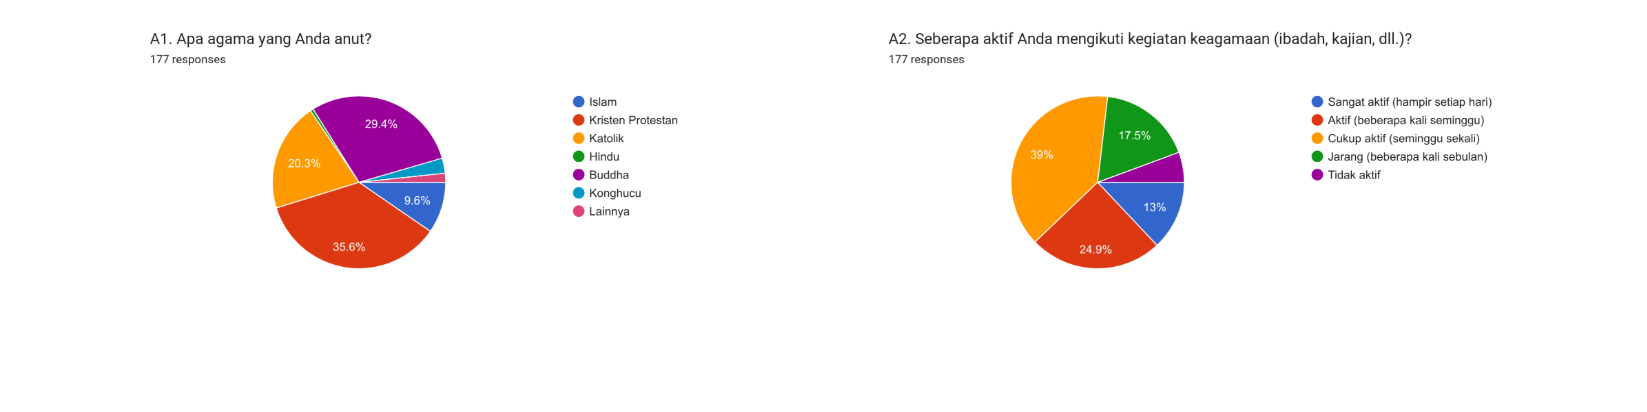
\includegraphics[width=\textwidth]{assets/respondent/distribusi_responden.png}
              \captionsetup{labelformat=empty}
               \caption[Diagram Distribusi Responden Berdasarkan Agama dan Keaktifan Kegiatan Keagamaan]{Gambar \ref{fig:PieChartpopulasi} Diagram distribusi responden berdasarkan agama dan keaktifan kegiatan keagamaan}
            \label{fig:PieChartpopulasi}
        \end{figure}

Berdasarkan Gambar 4.1, responden penelitian berasal dari latar belakang agama yang beragam. Mayoritas responden berasal dari agama Kristen Protestan sebesar 35,6%, diikuti oleh Buddha sebesar 29,4%, Katolik sebesar 20,3%, dan Islam sebesar 9,6%, sedangkan responden dari agama Hindu, Konghucu, dan agama lainnya memiliki persentase yang lebih kecil. Dari sisi keterlibatan dalam kegiatan keagamaan, mayoritas responden berada pada kategori cukup aktif sebesar 39%, diikuti kategori aktif sebesar 24,9%, jarang sebesar 17,5%, dan sangat aktif sebesar 13%.
        
Untuk memperoleh gambaran yang lebih jelas mengenai latar belakang agama responden, data distribusi responden berdasarkan agama disajikan pada Tabel 4.1.

\begin{table}[H]
\centering
\captionsetup{labelformat=empty}
\caption[Distribusi Responden Berdasarkan Agama]{Tabel \ref{tab:Tabelagama} Distribusi responden berdasarkan agama}
\label{tab:Tabelagama}
\begin{tabular}{ |c|c| } 
\hline
\textbf{Agama} & \textbf{Persentase (\%)} \\
\hline
Kristen Protestan & 35,6 \\ 
\hline
Buddha & 29,4 \\
\hline
Katolik & 20,3 \\
\hline
Islam & 9,6 \\
\hline
Hindu, Konghucu, dan lainnya & 5,1 \\
\hline
Total & 100\\
 
\hline
\end{tabular}
\end{table}

  
Berdasarkan Tabel 4.1, terlihat bahwa responden didominasi oleh penganut agama Kristen Protestan dan Buddha. Keberagaman latar belakang agama tersebut memungkinkan penelitian memperoleh pandangan yang lebih luas mengenai hubungan antara nilai keagamaan dan sikap terhadap korupsi.

Selain latar belakang agama, tingkat keaktifan responden dalam mengikuti kegiatan keagamaan juga menjadi salah satu aspek yang diamati dalam penelitian ini. Distribusi responden berdasarkan tingkat keaktifan kegiatan keagamaan disajikan pada Tabel 4.2. 

\begin{table}[H]
\centering
\captionsetup{labelformat=empty}
\caption[Distribusi responden berdasarkan keaktifan kegiatan keagamaan]{Tabel \ref{tab:Tabelkeaktifan} Distribusi responden berdasarkan keaktifan kegiatan keagamaan}
\label{tab:Tabelkeaktifan}
\begin{tabular}{ |c|c| } 
\hline
\textbf{Tingkat Keaktifan} & \textbf{Persentase (\%)} \\
\hline
Sangat aktif & 13 \\ 
\hline
Aktif & 24,9 \\
\hline
Cukup aktif & 39 \\
\hline
Jarang & 17,5 \\
\hline
Tidak aktif & 5,6 \\
\hline
Total & 100\\
\hline
\end{tabular}
\end{table}

Berdasarkan Tabel 4.2, sebagian besar responden berada pada kategori cukup aktif hingga aktif dalam mengikuti kegiatan keagamaan. Temuan ini menunjukkan bahwa mayoritas responden masih memiliki keterlibatan yang cukup rutin dalam aktivitas keagamaan, sehingga pandangan yang diberikan dalam kuesioner diharapkan cukup merepresentasikan pemahaman keagamaan yang dimiliki responden.

Setelah mengetahui karakteristik responden, analisis dilanjutkan pada hasil jawaban kuesioner yang berkaitan dengan pengetahuan dan pandangan responden mengenai korupsi dalam perspektif agama. Pertanyaan yang diberikan bertujuan untuk mengukur tingkat pemahaman responden mengenai larangan korupsi dalam agama, keberadaan sanksi moral atau spiritual bagi pelaku korupsi, serta paparan responden terhadap materi atau ceramah antikorupsi. 

Frekuensi jawaban responden pada pertanyaan pengetahuan dasar mengenai pandangan agama terhadap korupsi disajikan pada Tabel 4.3. 

\begin{table}[h]
\centering
\captionsetup{labelformat=empty}
\caption[Distribusi Jawaban Ya atau Tidak pada Pertanyaan Pengetahuan]{Tabel \ref{tab:Tabelpengetahuan} Distribusi jawaban ya atau tidak pada pertanyaan pengetahuan}
\label{tab:Tabelpengetahuan}
\begin{tabular}{ |c|p{8cm}|c|c| } 
\hline
\textbf{Kode} & \textbf{Pernyataan} & \textbf{Ya (\%)} & \textbf{Tidak (\%)} \\
\hline
B1 & Tahu agama melarang korupsi secara eksplisit & 95,5 & 4,5 \\ 
\hline
B2 & Pernah mendengar ceramah antikorupsi & 81,4 & 18,6 \\
\hline
B3 & Tahu adanya sanksi moral atau spiritual untuk pelaku korupsi & 94,4 & 5,6 \\
\hline
\end{tabular}
\end{table}

Data pada Tabel 4.3 menunjukkan bahwa mayoritas responden mengetahui bahwa agama mereka secara eksplisit melarang tindakan korupsi. Sebagian besar responden juga memahami adanya konsekuensi moral maupun spiritual yang dapat diterima oleh pelaku korupsi. Namun demikian, masih terdapat sejumlah responden yang belum pernah memperoleh ceramah atau pembinaan khusus mengenai antikorupsi. Temuan ini menunjukkan bahwa pemahaman dasar mengenai larangan korupsi dalam agama sudah cukup tinggi, tetapi upaya penyampaian nilai-nilai antikorupsi melalui kegiatan keagamaan masih dapat ditingkatkan.

Untuk memperoleh gambaran yang lebih mendalam mengenai sikap responden terhadap nilai agama dan perilaku antikorupsi, digunakan pertanyaan dengan skala Likert. Hasil rata-rata jawaban responden terhadap setiap pernyataan disajikan pada Tabel 4.4. 

\begin{table}[H]
    \centering
    \captionsetup{labelformat=empty}
    \caption[Skor rata-rata skala Likert sikap antikorupsi]{Tabel \ref{tab:Tabelhasilkuesioner} Skor rata-rata skala Likert sikap antikorupsi}
    \label{tab:Tabelhasilkuesioner}
    \begin{tabular}{ |c|p{8cm}|c|c| } 
    \hline
    \textbf{Kode} & \textbf{Pernyataan} & \textbf{Rata-Rata} & \textbf{Interpretasi} \\
    \hline
    B4 & Korupsi bertentangan dengan nilai-nilai agama saya & 4,62 & Sangat Setuju \\
    \hline
    B5 & Saya mengetahui tokoh agama yang aktif kampanye antikorupsi & 3,67 & Setuju \\
    \hline
    B6 & Ajaran agama telah memberikan pedoman yang jelas mengenai cara bekerja secara halal dan jujur & 4,56 & Sangat Setuju \\
    \hline
    C1 & Keyakinan agama menjadi alasan kuat menolak korupsi & 4,19 & Setuju \\
    \hline
    C2 & Saya merasa bertanggung jawab moral jika membiarkan korupsi & 3,93 & Setuju \\
    \hline
    C3 & Lembaga keagamaan berperan penting membangun budaya antikorupsi & 4,18 & Setuju \\
    \hline
    C4 & Orang taat beragama seharusnya tidak korupsi & 3,80 & Setuju \\
    \hline
    C5 & Ceramah antikorupsi berdampak nyata pada perilaku saya & 3,88 & Setuju \\
    \hline
    C6 & Rasa malu dan takut akibat spiritual mendorong saya jujur & 4,34 & Sangat Setuju \\
    \hline
    C7 & Pendidikan agama sejak kecil membentuk karakter antikorupsi & 4,27 & Setuju \\
    \hline
    C8 & Korupsi pasti membawa konsekuensi spiritual bagi pelakunya & 4,48 & Sangat Setuju \\
    \hline
    \end{tabular}
\end{table}

Berdasarkan Tabel 4.4, skor tertinggi diperoleh pada pernyataan bahwa korupsi bertentangan dengan nilai-nilai agama responden dengan nilai rata-rata sebesar 4,62. Pernyataan mengenai ajaran agama yang memberikan pedoman untuk bekerja secara halal dan jujur juga memperoleh skor yang tinggi, yaitu sebesar 4,56. Temuan ini menunjukkan bahwa responden memiliki keyakinan yang kuat bahwa agama mengajarkan nilai kejujuran dan menolak tindakan korupsi. 

Di sisi lain, skor yang relatif lebih rendah ditemukan pada pernyataan mengenai keberadaan tokoh agama yang aktif mengampanyekan antikorupsi dengan nilai rata-rata 3,67 serta dampak ceramah antikorupsi terhadap perilaku dengan nilai rata-rata 3,88. Hasil tersebut mengindikasikan bahwa meskipun pemahaman keagamaan mengenai korupsi sudah cukup baik, peran keteladanan tokoh agama dan efektivitas penyampaian pesan antikorupsi masih perlu diperkuat agar nilai-nilai agama dapat lebih nyata memengaruhi perilaku masyarakat. 

\subsection{Hasil Kualitatif}

Data kualitatif dalam penelitian ini diperoleh melalui wawancara dengan lima tokoh agama yang mewakili agama Buddha, Kristen, Katolik, Hindu, dan Islam. Wawancara dilakukan untuk memperoleh pemahaman yang lebih mendalam mengenai pandangan masing-masing agama terhadap tindakan korupsi, faktor-faktor yang menyebabkan praktik korupsi tetap terjadi di tengah masyarakat yang religius, serta peran agama dalam membentuk karakter dan moral antikorupsi. Hasil wawancara menunjukkan bahwa meskipun setiap agama memiliki ajaran dan pendekatan yang berbeda, seluruh narasumber sepakat bahwa korupsi merupakan tindakan yang bertentangan dengan nilai-nilai moral dan keagamaan. 

Narasumber dari agama Buddha menjelaskan bahwa korupsi merupakan pelanggaran terhadap Sila Kedua dalam Pancasila Buddhis, yaitu larangan mengambil sesuatu yang tidak diberikan atau bukan haknya. Tindakan korupsi dipandang berakar pada keserakahan dan kebodohan batin yang mendorong seseorang untuk mengabaikan nilai-nilai moral. Oleh karena itu, pencegahan korupsi perlu dilakukan melalui pengendalian diri, pengembangan rasa cukup, serta penerapan prinsip mata pencaharian benar dalam kehidupan sehari-hari. 

Pandangan yang serupa juga ditemukan dalam agama Kristen. Korupsi dipahami sebagai bentuk dosa karena berkaitan dengan tindakan mencuri dan kecintaan yang berlebihan terhadap uang. Menurut narasumber, umat Kristen perlu membangun sikap syukur, kejujuran, dan tanggung jawab dalam pekerjaan maupun kehidupan sosial. Selain itu, konsep menjadi “garam dan terang dunia” mengajarkan bahwa seseorang tidak hanya dituntut untuk menjauhi korupsi, tetapi juga menjadi teladan yang memberikan pengaruh positif bagi lingkungan sekitarnya. 

Sementara itu, narasumber dari agama Katolik menekankan bahwa korupsi tidak hanya merupakan kesalahan individu, tetapi juga termasuk dosa sosial karena dampaknya merugikan banyak orang dan menghambat terwujudnya kesejahteraan bersama. Oleh sebab itu, penghayatan iman tidak boleh berhenti pada praktik ritual keagamaan semata, melainkan perlu diwujudkan dalam kehidupan sosial melalui keberanian menolak gratifikasi, membiasakan perilaku jujur, dan mengutamakan kepentingan bersama di atas kepentingan pribadi. 

Dalam ajaran Hindu, korupsi dipahami sebagai tindakan yang bertentangan dengan Dharma karena melibatkan pengambilan hak yang bukan miliknya. Narasumber menjelaskan bahwa pencarian harta atau Artha harus selalu dilandasi oleh Dharma agar tidak berubah menjadi keserakahan yang merugikan orang lain. Selain itu, nilai Tri Kaya Parisudha yang menekankan kesucian pikiran, perkataan, dan perbuatan menjadi pedoman penting dalam membentuk perilaku yang jujur dan bertanggung jawab. 

\subsection{Pembahasan}
Hasil wawancara dan kuesioner menunjukkan adanya pola yang konsisten, yaitu seluruh agama memiliki landasan moral yang kuat dalam menolak tindakan korupsi. Korupsi dipahami sebagai tindakan mengambil hak orang lain secara tidak sah, baik dalam bentuk uang, waktu, jabatan, maupun kewenangan. Pandangan ini muncul dalam wawancara dengan tokoh agama Buddha, Kristen, Katolik, Hindu, dan Islam. Dengan demikian, secara normatif agama memiliki posisi yang jelas dalam menolak korupsi.

Meskipun demikian, hasil penelitian menunjukkan adanya kesenjangan antara pengetahuan agama dan penerapan moral dalam kehidupan nyata. Hal ini terlihat dari tingginya persentase responden yang mengetahui bahwa agama melarang korupsi, tetapi skor mengenai dampak ceramah antikorupsi terhadap perilaku masih lebih rendah dibandingkan skor keyakinan teologis. Kondisi ini menunjukkan bahwa masyarakat tidak hanya membutuhkan pengetahuan bahwa korupsi itu salah, tetapi juga membutuhkan pembinaan moral yang mampu menjawab situasi konkret dalam kehidupan sehari-hari.

Kesenjangan tersebut juga terlihat dari rendahnya skor mengenai pengetahuan responden terhadap tokoh agama yang aktif mengampanyekan antikorupsi. Artinya, masyarakat belum cukup terekspos pada figur keteladanan yang secara nyata menyuarakan nilai antikorupsi di ruang publik. Padahal, tokoh agama memiliki peran penting sebagai panutan moral yang dapat membantu masyarakat menerjemahkan ajaran agama menjadi tindakan nyata.

Berdasarkan hasil tersebut, penanaman moral antikorupsi tidak cukup dilakukan melalui ceramah yang hanya bersifat normatif. Pembinaan keagamaan perlu dikembangkan menjadi diskusi moral yang lebih kontekstual, misalnya dengan membahas kasus suap, gratifikasi, manipulasi data, titip absen, plagiarisme, dan bentuk ketidakjujuran lain yang dekat dengan kehidupan masyarakat. Dengan demikian, nilai agama tidak hanya dipahami sebagai aturan, tetapi juga menjadi dasar dalam mengambil keputusan moral.

\newpage

Selain itu, pendidikan antikorupsi berbasis nilai agama perlu diterapkan sejak dini melalui keluarga, sekolah, lembaga keagamaan, dan masyarakat. Keluarga dapat membiasakan kejujuran dalam kehidupan sehari-hari, sekolah dapat menanamkan integritas melalui aturan dan pembelajaran, sedangkan lembaga keagamaan dapat memperkuat kesadaran moral melalui pembinaan yang relevan dengan realitas sosial. Kolaborasi berbagai pihak tersebut diperlukan agar nilai kejujuran, tanggung jawab, dan integritas dapat benar-benar diterapkan dalam kehidupan masyarakat.

\subsection{Dokumentasi Kegiatan}

Dokumentasi kegiatan disajikan sebagai pelengkap laporan untuk memberikan gambaran mengenai pelaksanaan kegiatan yang telah dilakukan. Dokumentasi ini menunjukkan keterlibatan para narasumber dalam proses pengumpulan data serta menjadi bukti pelaksanaan kegiatan yang mendukung penyusunan laporan. Salah satu dokumentasi kegiatan dapat dilihat pada Gambar 4.2.

\begin{figure}[H]
            \centering
            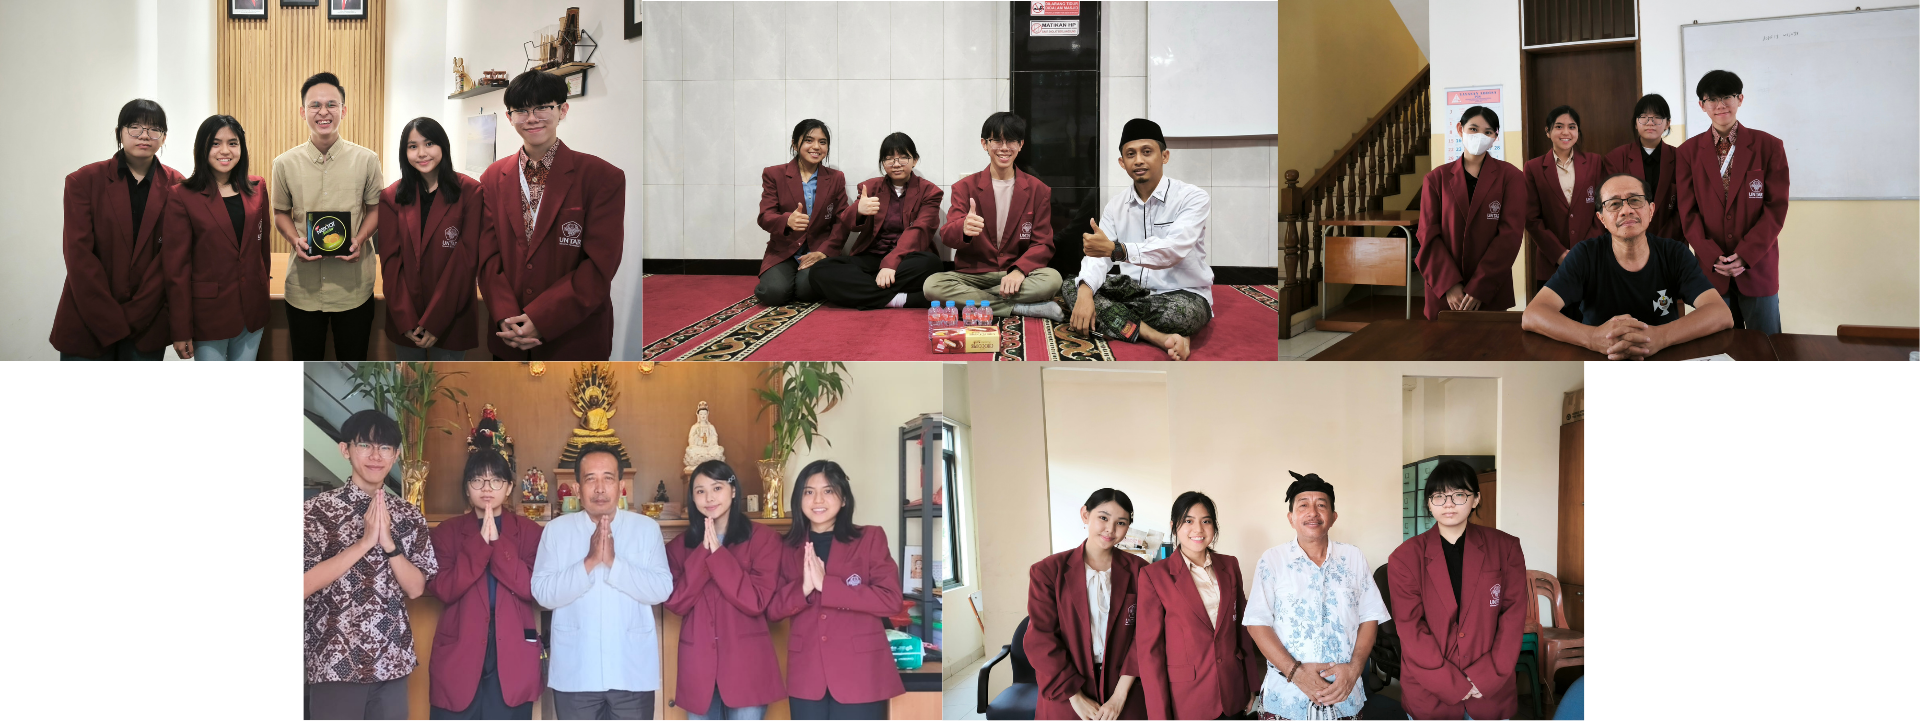
\includegraphics[width=10cm]{assets/documentation/foto_narasumber_all.png}
              \captionsetup{labelformat=empty}
               \caption[Foto bersama para narasumber]{Gambar \ref{fig:FOTONARASUMBER} Foto bersama para narasumber kegiatan wawancara}
            \label{fig:FOTONARASUMBER}
        \end{figure}

Dokumentasi kegiatan menunjukkan pelaksanaan wawancara bersama para narasumber dari berbagai latar belakang agama. Foto bersama narasumber menjadi bukti bahwa kegiatan studi lapangan telah dilaksanakan secara langsung. Melalui kegiatan wawancara ini, tim peneliti memperoleh pemahaman yang lebih luas mengenai bagaimana masing-masing agama memandang tindakan korupsi dan bagaimana nilai keagamaan dapat digunakan untuk menanamkan moral antikorupsi kepada masyarakat.
    
Kegiatan wawancara juga memperlihatkan bahwa isu korupsi tidak hanya dapat dibahas dari sudut pandang hukum, tetapi juga dari sudut pandang moral dan spiritual. Setiap narasumber memberikan penekanan yang berbeda sesuai dengan ajaran agamanya, namun seluruhnya sepakat bahwa korupsi merupakan tindakan yang merusak nilai kejujuran, tanggung jawab, dan keadilan sosial. Oleh karena itu, dokumentasi kegiatan ini menjadi bagian penting dalam laporan karena menunjukkan keterlibatan langsung narasumber dalam memberikan perspektif keagamaan terhadap moral antikorupsi.

    \newpage

\renewcommand\thesection{5}
\renewcommand\thesubsection{\arabic{subsection}}

\counterwithin{subsection}{section}
\setcounter{subsection}{0}

\begin{center}
    \section*{\textbf{BAB V \\ KESIMPULAN DAN SARAN}}
    \addcontentsline{toc}{section}{BAB V \quad KESIMPULAN DAN SARAN}
\end{center}

\subsection{Kesimpulan}
\hspace{0.5cm}Berdasarkan hasil kegiatan yang telah dilaksanakan, maka dapat ditarik kesimpulan bahwa agama memiliki peran penting dalam menanamkan moral antikorupsi kepada masyarakat. Hasil kuesioner menunjukkan bahwa mayoritas responden mengetahui bahwa agama mereka melarang korupsi secara eksplisit dan memahami adanya sanksi moral atau spiritual bagi pelaku korupsi. Hal ini menunjukkan bahwa pengetahuan keagamaan masyarakat mengenai larangan korupsi sudah cukup tinggi. Selain itu, hasil wawancara dengan tokoh agama Buddha, Kristen, Katolik, Hindu, dan Islam menunjukkan bahwa seluruh agama memandang korupsi sebagai pelanggaran moral yang serius karena berkaitan dengan tindakan mengambil hak orang lain secara tidak sah.

\hspace{0.5cm}Meskipun demikian, kegiatan ini juga menemukan adanya kesenjangan antara pengetahuan agama dan penerapan moral dalam kehidupan nyata. Masyarakat mengetahui bahwa korupsi merupakan tindakan yang salah, tetapi nilai tersebut belum selalu diwujudkan dalam perilaku sehari-hari. Hal ini terlihat dari skor mengenai dampak ceramah antikorupsi terhadap perilaku yang masih lebih rendah dibandingkan skor keyakinan bahwa korupsi bertentangan dengan nilai agama. Selain itu, pengetahuan responden mengenai tokoh agama yang aktif mengampanyekan antikorupsi juga masih belum terlalu tinggi. Dengan demikian, penanaman moral antikorupsi tidak cukup hanya dilakukan melalui penyampaian ajaran agama secara normatif, tetapi perlu diperkuat melalui pembinaan moral yang lebih kontekstual, keteladanan tokoh agama, serta pendidikan antikorupsi berbasis nilai agama.


\subsection{Saran}
\hspace{0.5cm} 
Berdasarkan hasil kegiatan yang telah dilakukan, terdapat beberapa saran yang dapat diberikan. Pertama, lembaga keagamaan diharapkan tidak hanya menyampaikan ajaran mengenai larangan korupsi secara umum, tetapi juga membahas kasus-kasus nyata yang dekat dengan kehidupan masyarakat, seperti suap, gratifikasi, penyalahgunaan wewenang, manipulasi data, mencontek, dan plagiarisme. Kedua, tokoh agama perlu lebih aktif hadir sebagai figur teladan dalam menyuarakan nilai kejujuran, tanggung jawab, dan integritas, baik di lingkungan keagamaan maupun di ruang publik. Ketiga, lembaga pendidikan, keluarga, dan masyarakat perlu bekerja sama dalam menanamkan pendidikan antikorupsi sejak dini agar nilai agama tidak hanya dipahami sebagai aturan, tetapi juga menjadi dasar dalam mengambil keputusan moral.

\hspace{0.5cm} 
Penelitian ini juga memiliki keterbatasan karena responden kuesioner belum sepenuhnya mewakili seluruh kelompok masyarakat secara merata. Selain itu, wawancara hanya dilakukan kepada lima tokoh agama sehingga masih terdapat kemungkinan untuk memperluas sudut pandang dengan melibatkan lebih banyak narasumber dari berbagai lembaga keagamaan, pendidikan, maupun masyarakat umum. Oleh karena itu, penelitian selanjutnya diharapkan dapat menggunakan jumlah responden yang lebih besar, latar belakang responden yang lebih beragam, serta pembahasan yang lebih mendalam mengenai pengaruh pendidikan agama terhadap pembentukan perilaku antikorupsi dalam kehidupan sehari-hari.

    \newpage

\renewcommand{\bibsection}{}

\begin{center}
    \addcontentsline{toc}{section}{DAFTAR PUSTAKA}
    \section*{\textbf{DAFTAR PUSTAKA}}
\end{center}

\vspace{1cm}

\nocite{*}
\bibliographystyle{apalike}
\bibliography{contents/Daftar_Pustaka}
    \counterwithin{table}{section}

\newpage

% Set section counter to 5
\setcounter{section}{5}
\renewcommand\thesection{\arabic{section}}
\renewcommand\thesubsection{\arabic{subsection}}

\label{lampiran1}
\begin{center}
    \phantomsection
    \addcontentsline{toc}{section}{LAMPIRAN I SURAT KETERANGAN}
    \section*{\textbf{LAMPIRAN I SURAT KETERANGAN}}
\end{center}
            \begin{secondfigure}[H]
                \centering
                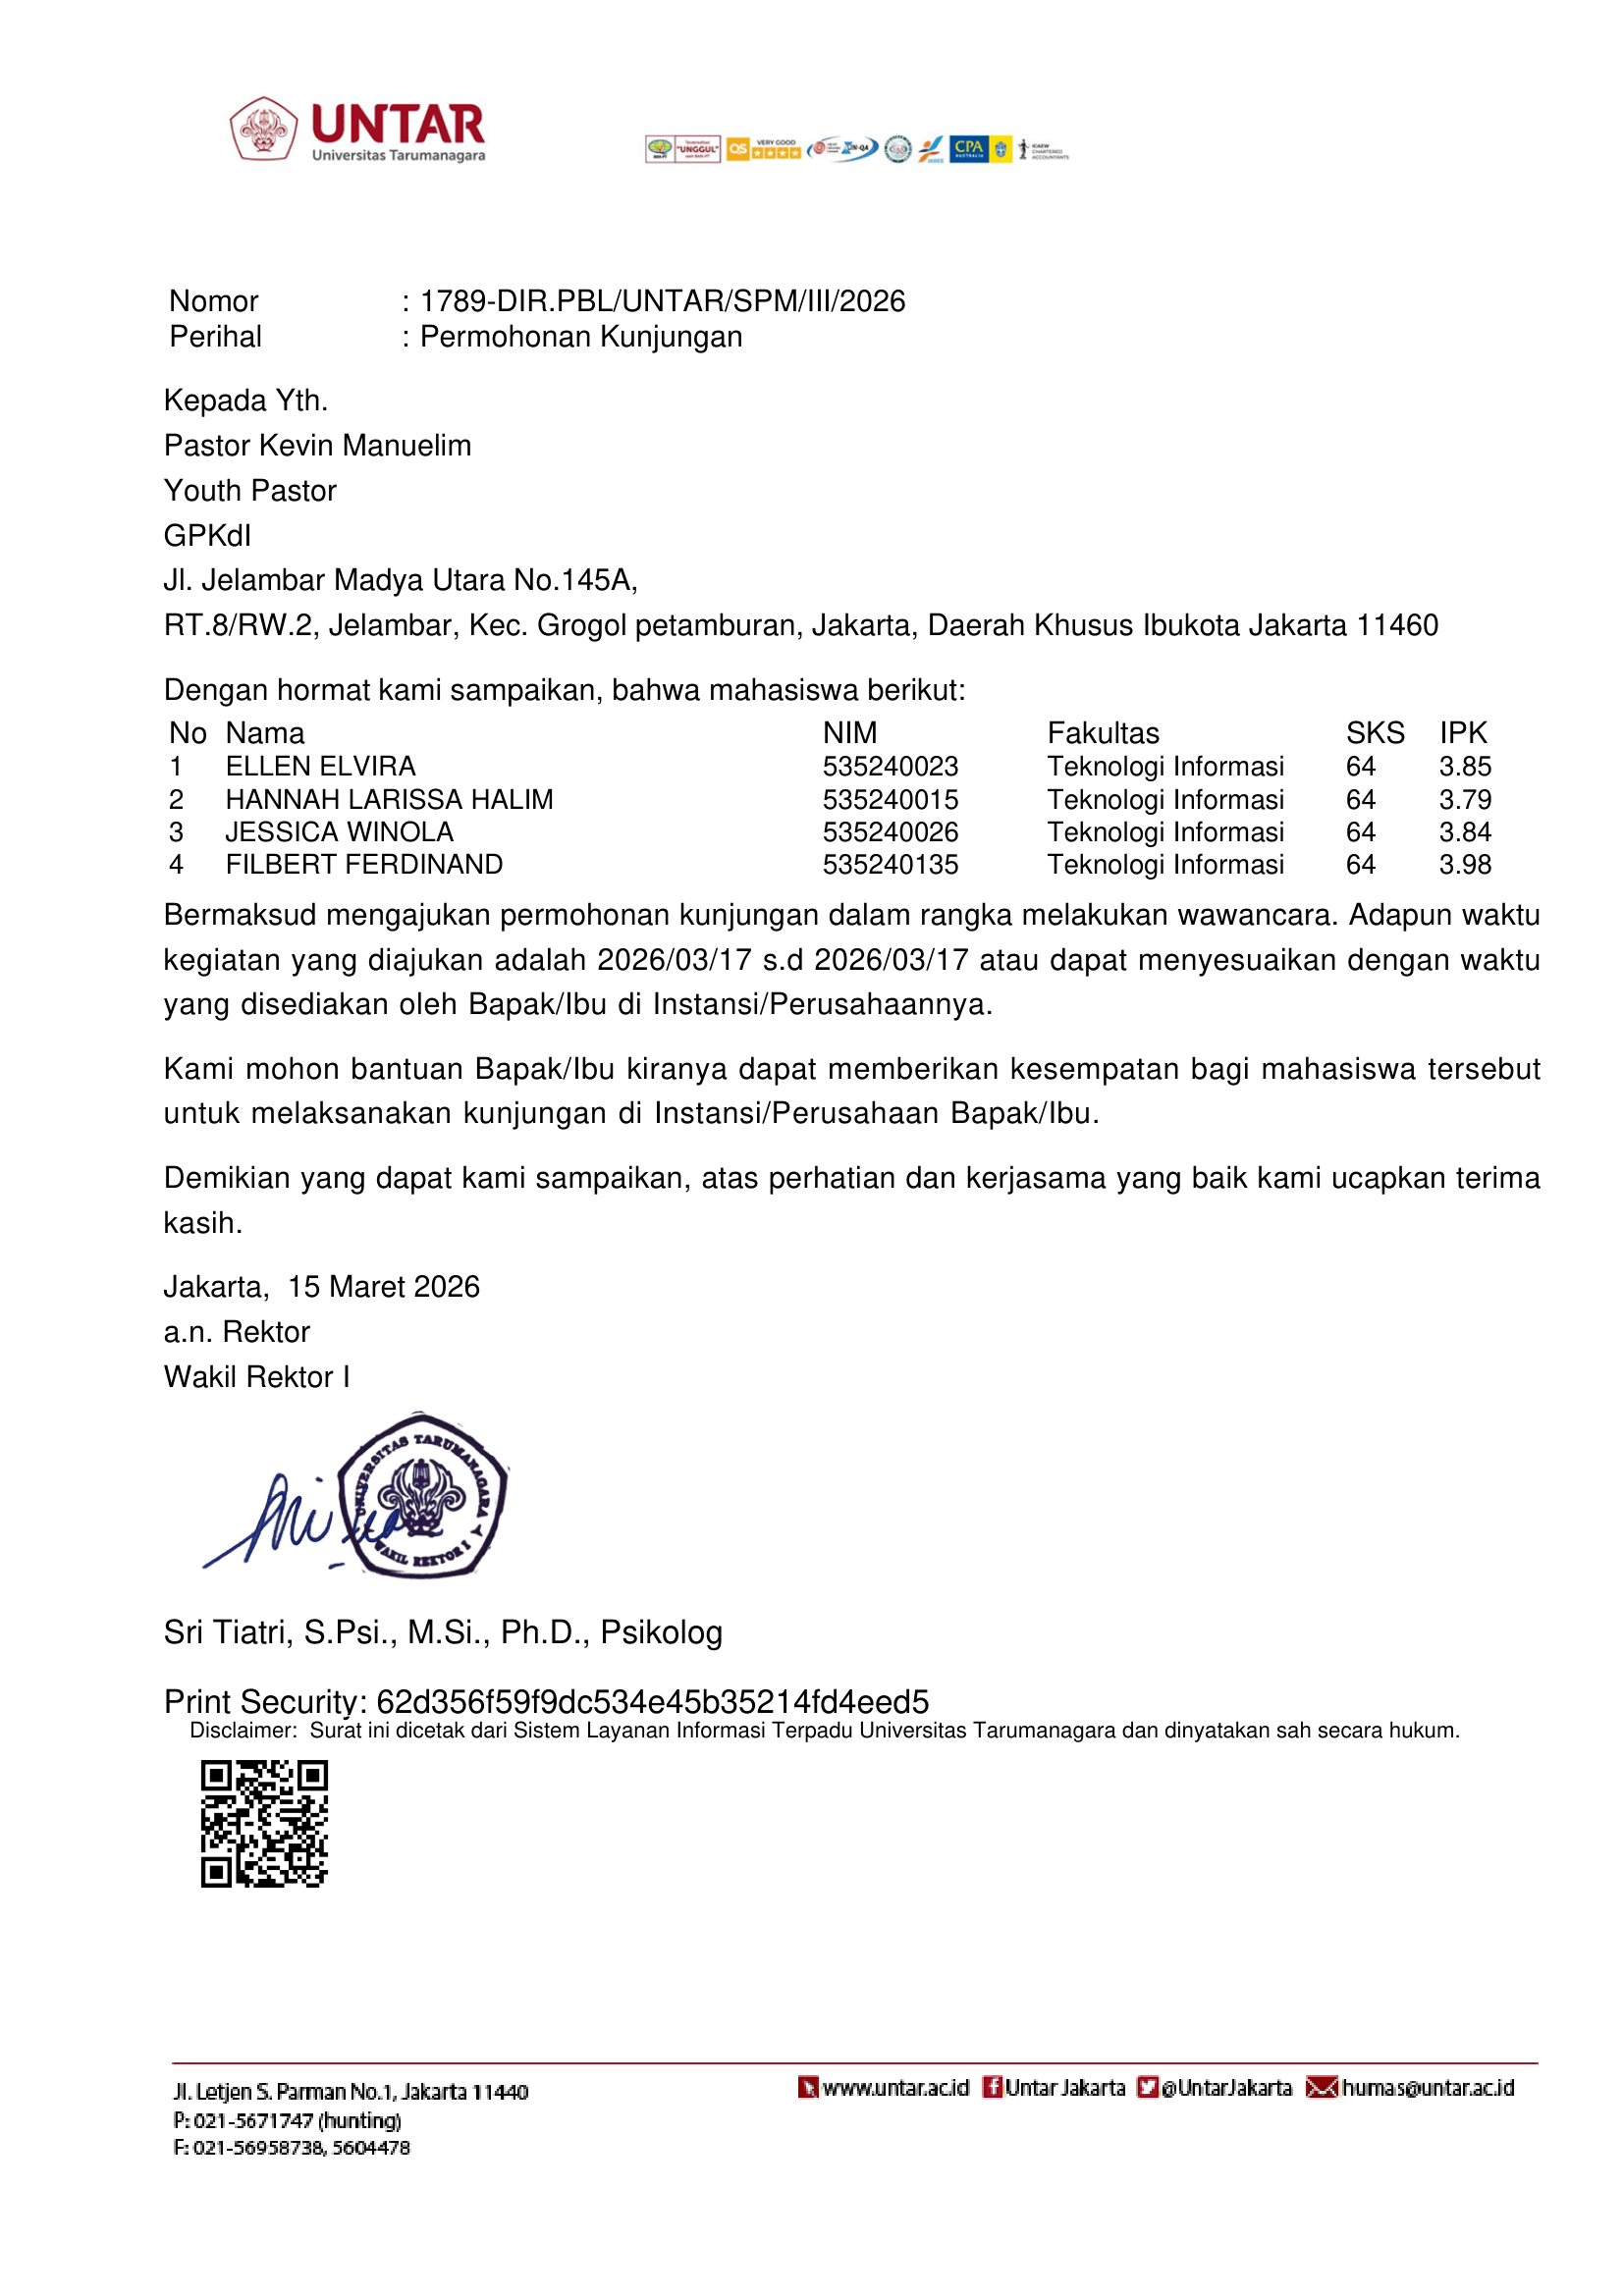
\includegraphics[width = 13cm]{assets/attachments/surat premohonan kunjungan GPKdI .png}
                \captionsetup{labelformat=empty}
                % \caption[Lampiran 2 Surat Permohonan LINTAR]{Lampiran 2 Surat Permohonan LINTAR}
                \label{fig:SuratLINTAR}
            \end{secondfigure}
            \begin{secondfigure}[H]
                \centering
                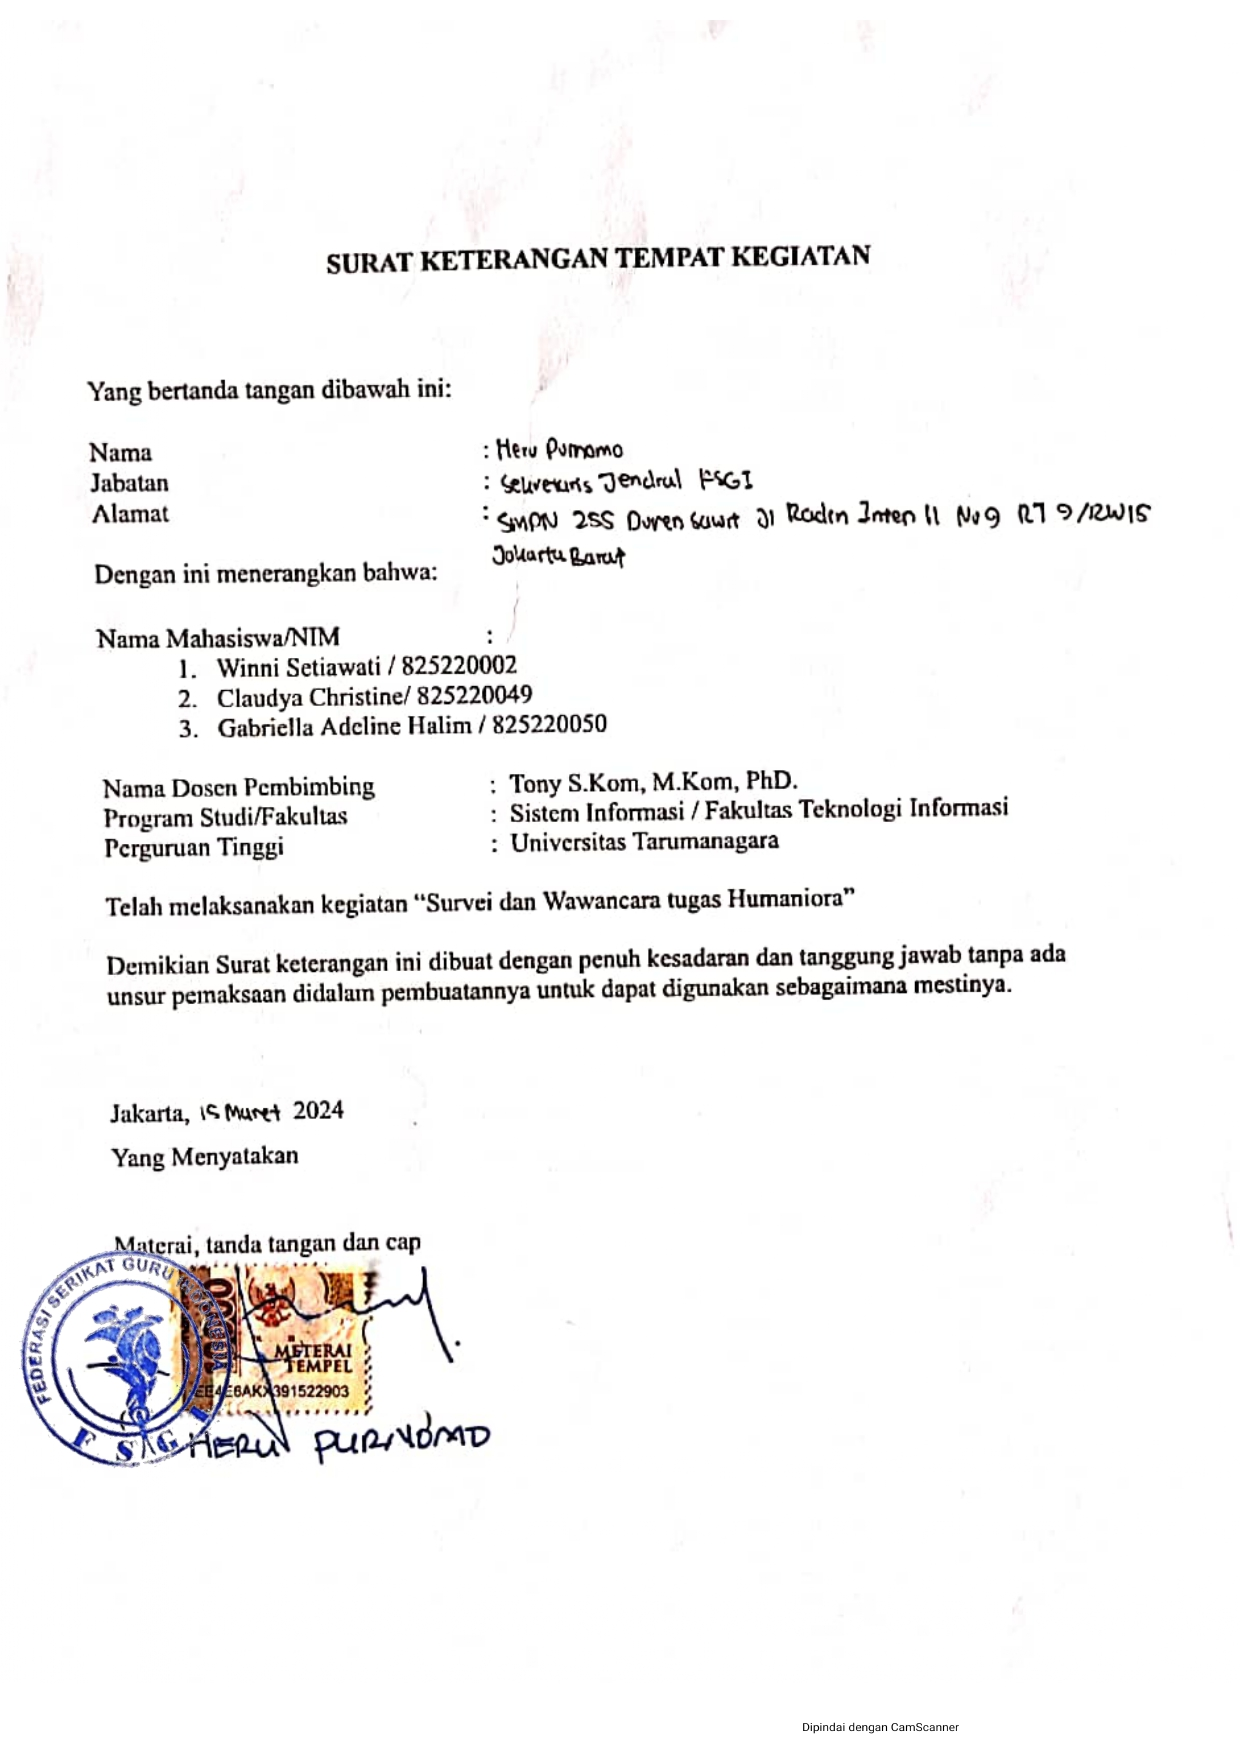
\includegraphics[width = 13cm]{assets/attachments/ttd surat keterangan wawancara_page-0001.jpg}
                \captionsetup{labelformat=empty}
                % \caption[Lampiran 1 Surat Keterangan Tempat Kegiatan]{Lampiran 1 Surat Keterangan Tempat Kegiatan}
                \label{fig:SuratKegiatan}
            \end{secondfigure}
           
\newpage
\label{lampiran2}
\begin{center}
    \addcontentsline{toc}{section}{LAMPIRAN II DOKUMENTASI PELAKSANAAN KEGIATAN}
    \section*{\textbf{LAMPIRAN II DOKUMENTASI PELAKSANAAN KEGIATAN}}
\end{center}
  \begin{secondfigure}[H]
        \centering
        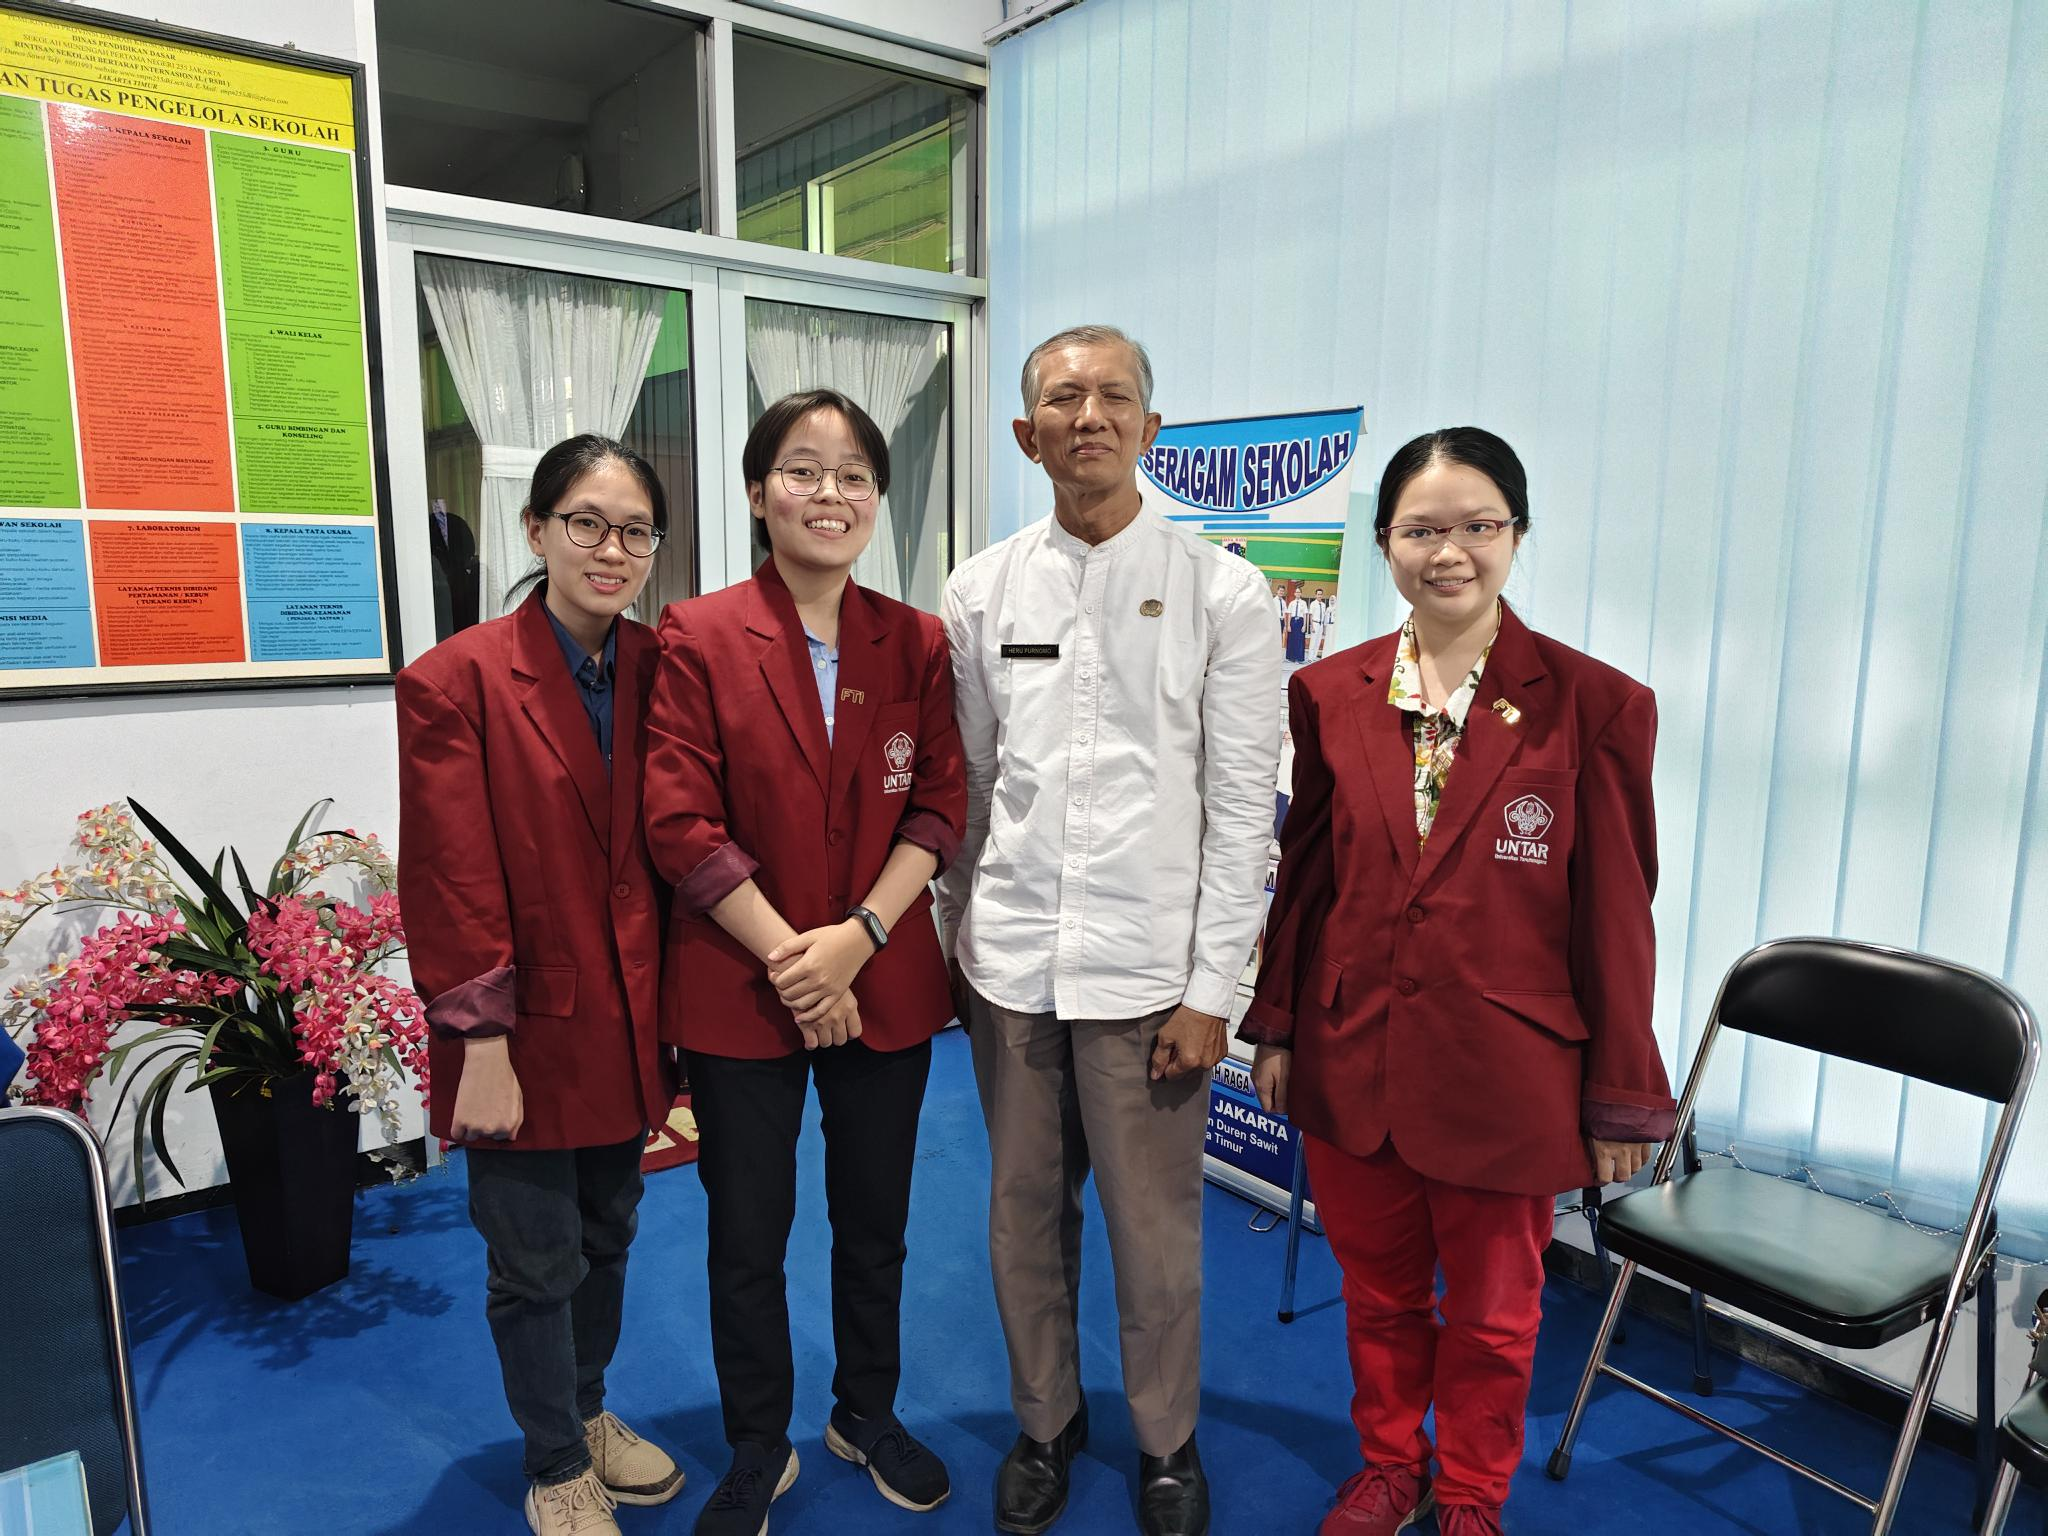
\includegraphics[width = 8cm]{assets/documentation/2 photos added (1).jpeg}
        \captionsetup{labelformat=empty}
        % \caption[Lampiran 3 Wawancara dengan Pak Heru Purnomo Sekretaris Jendral FSGI}
        \label{fig:FotoWawancaraFSGI}
    \end{secondfigure}

    \begin{secondfigure}[H]
        \centering
        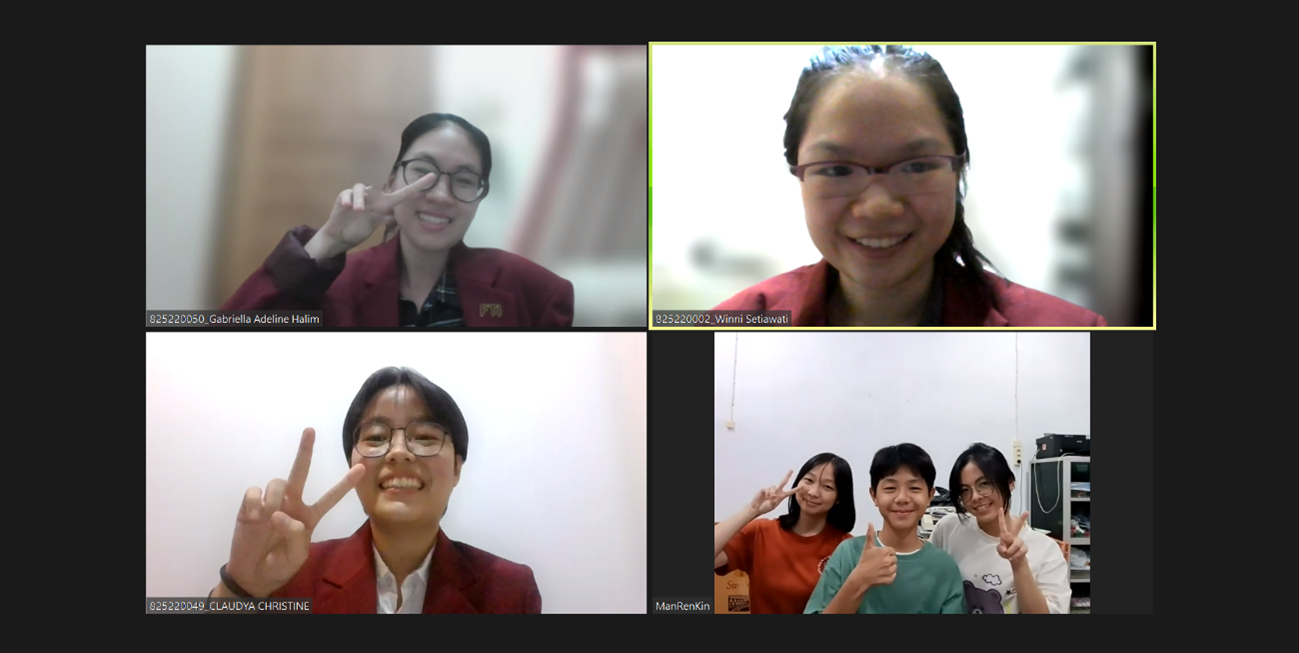
\includegraphics[width = 10cm]{assets/documentation/Picture1wawancarasiswa.png}
        \captionsetup{labelformat=empty}
         % \caption[Lampiran 4 Wawancara dengan siswa]{Lampiran 4 Foto Wawancara dengan siswa}
        \label{fig:FotoWawancarasiswa}
    \end{secondfigure}

    \begin{secondfigure}[H]
        \centering
        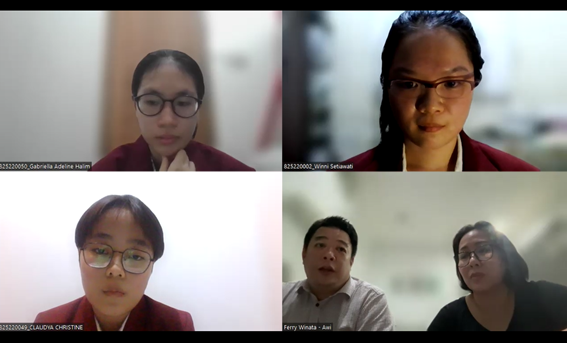
\includegraphics[width = 10cm]{assets/documentation/Picture2wawancaraortu.png}
        \captionsetup{labelformat=empty}
         % \caption[Lampiran 5 Foto wawancara dengan orang tua siswa ]{Lampiran 5 Foto wawancara dengan orang tua siswa }
        \label{fig:FotoWawancaraOrtu}
    \end{secondfigure}

        \begin{minipage}{1\linewidth}
        \begin{minipage}[hb]{0.5\linewidth}
            \begin{secondfigure}[H]
                \centering
                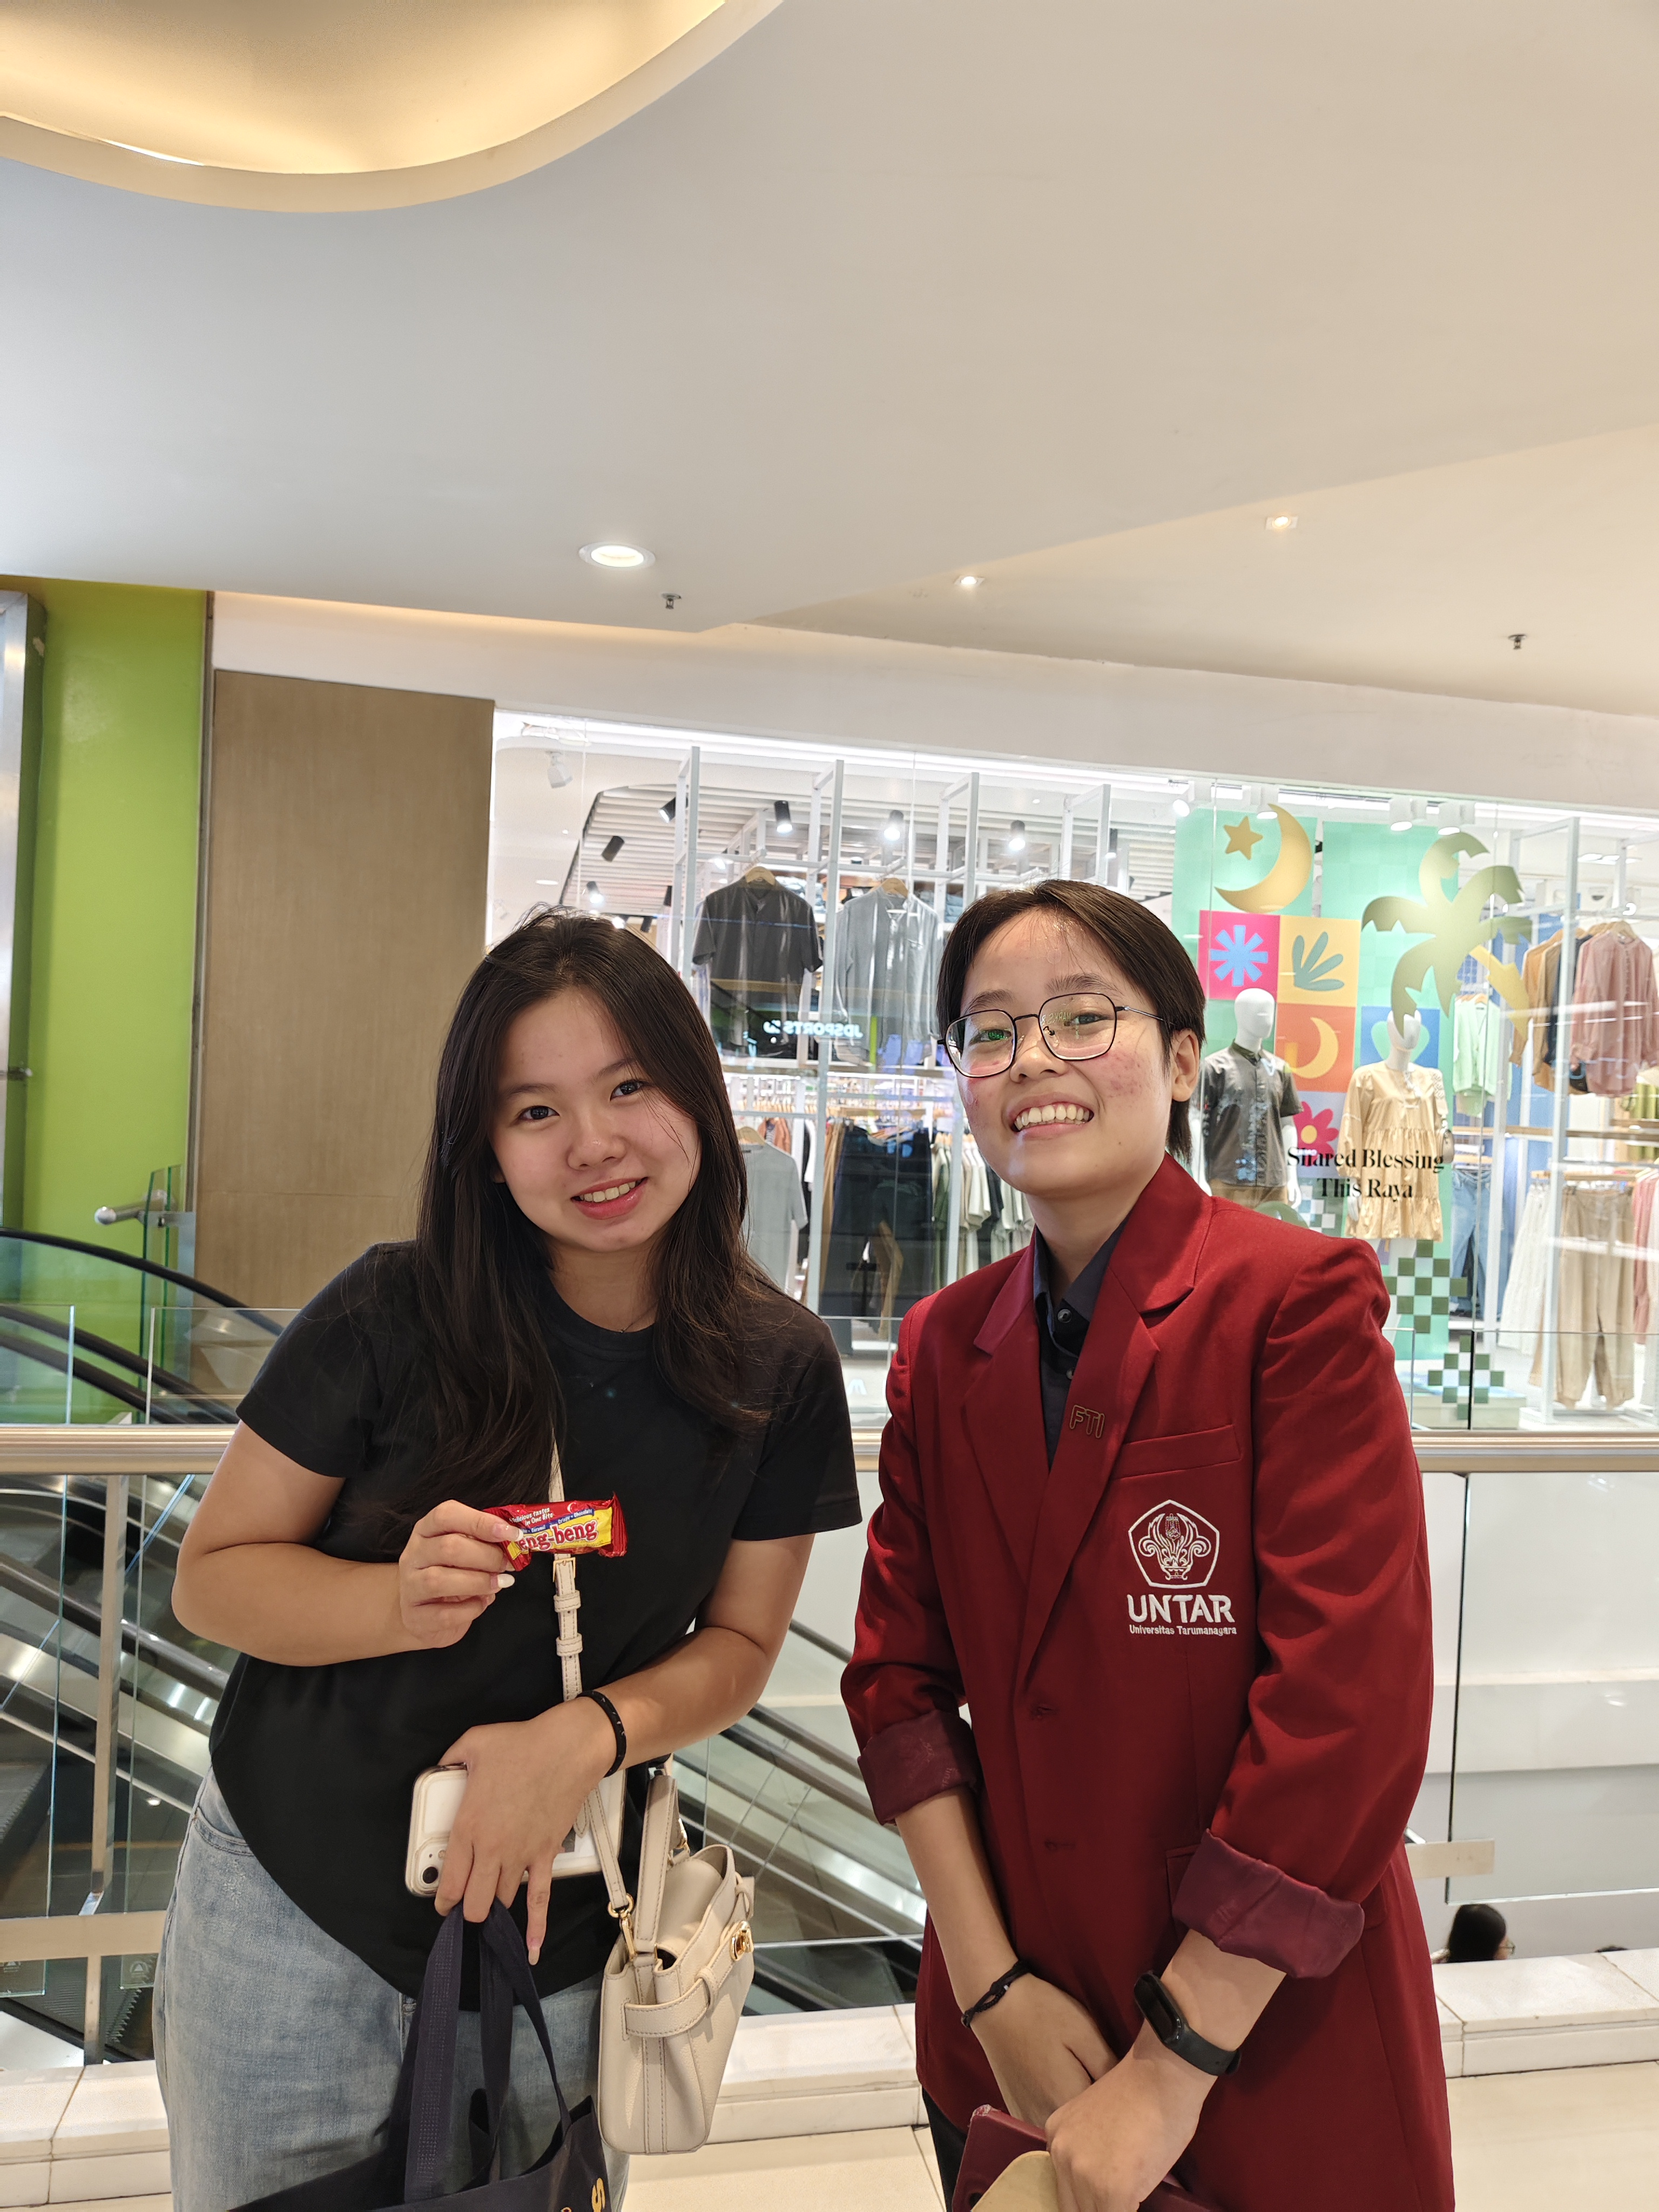
\includegraphics[width = 7cm]{assets/documentation/IMG_20240312_132116.jpg}
                \captionsetup{labelformat=empty}
                 % \caption[Lampiran 6 wawancara masyarakat umum 1]{Lampiran 6 wawancara masyarakat umum 1}
                \label{fig:wawancaramasya1}
            \end{secondfigure}
        \end{minipage}
        \hfill
        \hspace{0.3cm}
        \begin{minipage}[hb]{0.5\linewidth}
                 \begin{secondfigure}[H]
                    \centering
                    \includegraphics[width = 7cm]{assets/documentation/IMG_20240312_134754.jpg}
                    \captionsetup{labelformat=empty}
                     % \caption[Lampiran 7 Foto wawancara masyarakat 2]{Lampiran 7 Foto wawancara masyarakat 2}
                    \label{fig:wawancaramasya2}
                \end{secondfigure}
        \end{minipage}
    \end{minipage}
    
        \begin{secondfigure}[H]
            \centering
            \includegraphics[width = 11cm]{assets/documentation/IMG_20240312_131239.jpg }
            \captionsetup{labelformat=empty}
            % \caption[Lampiran 8 Foto wawancara masyarakat 3}
            \label{fig:wawancaramasya3}
        \end{secondfigure} 

\vspace*{2.cm}



\newpage
\label{lampiran3}
\setcounter{table}{0}

\begin{center}
    \addcontentsline{toc}{section}{LAMPIRAN III DAFTAR PERTANYAAN}
    \section*{\textbf{LAMPIRAN III DAFTAR PERTANYAAN DAN HASIL JAWABAN KUESIONER}}
\end{center}

\hspace{5cm}

\begin{table}[h]

\captionsetup{labelformat=empty}
\caption[Persentase sebaran jawaban kuesioner berdasarkan kategori pertanyaan pengetahuan responden terhadap pengertian, penyebab, dampak, tata laksana \textit{cyberbullying} ada anak usia sekolah]{Tabel \ref{tab:TabelhasilkuesionerX1} Persentase sebaran jawaban kuesioner berdasarkan kategori pertanyaan pengetahuan responden terhadap pengertian, penyebab, dampak, tata laksana \textit{cyberbullying} ada anak usia sekolah}
\label{tab:TabelhasilkuesionerX1}

\begin{tabular}{ |p{1.4cm}|p{5.4cm}|p{1.3cm}|p{1cm}|p{1cm}|p{1cm}|p{1cm}| } 
\hline
\centering \textbf{Kategori Variabel} & \centering \textbf{Butir Pertanyaan} & \centering \textbf{Sangat Tidak Setuju (\%)} & \centering \textbf{Tidak Setuju (\%)} & \centering \textbf{Netral (\%)} & \centering \textbf{Setuju (\%)} &  \textbf{\centering Sangat Setuju (\%)} \\
\hline
\multicolumn{7}{|c|}{X1 : Pengetahuan responden terhadap pengertian, penyebab, dampak, tata laksana \textit{cyberbullying} }\\
\multicolumn{7}{|c|}{ada anak usia sekolah} \\
\hline
X1 & Saya mengetahui apa itu \textit{cyberbullying}. & 12,2 & 3,6 & 11,5 & 43,5 & 29,5 \\
\hline
X1 & Saya mengetahui penyebab \textit{cyberbullying} pada siswa bisa terjadi. & 7,2 & 3,6 & 15,1 & 54,7 & 19,4 \\
\hline
X1 & Saya mengetahui dampak yang dihasilkan oleh \textit{cyberbullying} terhadap korban maupun pelaku. & 7,9 & 2,9 & 8,6 & 52,5 & 28,1 \\
\hline
X1 & \textit{Cyberbullying} merupakan kelanjutan dari \textit{bullying} konvensional dengan menggunakan media sosial/alat media \textit{virtual}. & 7,9 & 2,2 & 10,8 & 51,1 & 28,1 \\
\hline
X1 & Saya sering melihat atau mendengar kasus \textit{cyberbullying} di lingkungan sekolah atau masyarakat. & 7,2 & 8,6 & 17,3 & 46 & 20,9 \\
\hline
X1 & Saya mengetahui tindakan yang harus saya ambil ketika seorang siswa sedang menjadi korban \textit{cyberbullying}. & 2,2 & 7,2 & 25,2 & 51,8 & 13,7 \\
\hline 

\end{tabular}
\end{table}

\begin{table}[h]

\captionsetup{labelformat=empty}
\caption[Persentase sebaran jawaban kuesioner berdasarkan kategori pertanyaan tingkat kepuasan responden terhadap upaya sekolah dan mengerti pentingnya kolaborasi sosial berjenjang]{Tabel \ref{tab:TabelhasilkuesionerX2} Persentase sebaran jawaban kuesioner berdasarkan kategori pertanyaan tingkat kepuasan responden terhadap upaya sekolah dan mengerti pentingnya kolaborasi sosial berjenjang}
\label{tab:TabelhasilkuesionerX2}
\begin{tabular}{ |p{1.4cm}|p{5.4cm}|p{1.3cm}|p{1cm}|p{1cm}|p{1cm}|p{1cm}| } 
\hline
\centering \textbf{Kategori Variabel} & \centering \textbf{Butir Pertanyaan} & \centering \textbf{Sangat Tidak Setuju (\%)} & \centering \textbf{Tidak Setuju (\%)} & \centering \textbf{Netral (\%)} & \centering \textbf{Setuju (\%)} &  \textbf{\centering Sangat Setuju (\%)} \\
\hline
\multicolumn{7}{|c|}{X2 : Tingkat kepuasan responden terhadap upaya sekolah dan mengerti pentingnya kolaborasi } \\
\multicolumn{7}{|c|}{sosial berjenjang } \\

\hline
X2 & Saya mengetahui tindakan yang harus saya ambil ketika seorang siswa sedang menjadi korban \textit{cyberbullying}. & 6,5 & 26,6 & 33,1 & 23,7 & 10,1 \\
\hline
X2 & Pihak sekolah telah mengupayakan untuk meminimalisir kejadian \textit{cyberbullying} siswa di lingkungan sekolah berupa kebijakan memasukkan ponsel siswa ke dalam \textit{box} selama tidak dibutuhkan saat pelajaran. Menurut saya kebijakan tersebut baik untuk diterapkan. & 5,8 & 11,5 & 23,7 & 44,6 & 14,4 \\
\hline
X2 & Menurut saya penyamaan persepsi mengenai pencegahan \textit{cyberbullying} memerlukan kolaborasi antara sekolah, masyarakat, pemerintah, dan pihak terkait lainnya. & 0 & 2,2 & 7,2 & 46,8 & 43,9 \\
\hline
X2 & Saya merasa kolaborasi antar sekolah, masyarakat, pemerintah, dan pihak terkait lainnya untuk mencegah dan menganggulangi \textit{cyberbullying} pada anak sekolah sudah baik. & 2,9 & 28,8 & 36,7 & 24,5 & 7,2 \\
\hline
X2 & Menurut saya sosialisasi kepada orang tua dan anak-anak didik mengenai kebijakan penggunaan ponsel yang terhubung internet di lingkungan sekolah sudah baik. & 3,6 & 23 & 34,5 & 29,5 & 9,4 \\
\hline
X2 & Saya merasa literasi \textit{digital} dapat mengurangi dampak negatif penggunaan teknologi \textit{digital} pada siswa. & 0 & 6,5 & 29,5 & 46 & 18 \\
\hline
\end{tabular}
\end{table}

\begin{table}[h]

\captionsetup{labelformat=empty}
\caption[Persentase sebaran jawaban kuesioner berdasarkan kategori pertanyaan kesediaan responden melakukan perilaku bela negara untuk mencegah terjadinya \textit{cyberbullying} pada anak tingkat sekolah]{Tabel \ref{tab:TabelhasilkuesionerX3} Persentase sebaran jawaban kuesioner berdasarkan kategori pertanyaan kesediaan responden melakukan perilaku bela negara untuk mencegah terjadinya \textit{cyberbullying} pada anak tingkat sekolah}
\label{tab:TabelhasilkuesionerX3}
\begin{tabular}{ |p{1.4cm}|p{5.4cm}|p{1.3cm}|p{1cm}|p{1cm}|p{1cm}|p{1cm}| } 
\hline
\centering \textbf{Kategori Variabel} & \centering \textbf{Butir Pertanyaan} & \centering \textbf{Sangat Tidak Setuju (\%)} & \centering \textbf{Tidak Setuju (\%)} & \centering \textbf{Netral (\%)} & \centering \textbf{Setuju (\%)} &  \textbf{\centering Sangat Setuju (\%)} \\
\hline
\multicolumn{7}{|c|}{X3 : Kesediaan responden melakukan perilaku bela negara untuk mencegah terjadinya } \\
\multicolumn{7}{|c|}{\textit{cyberbullying} pada anak tingkat sekolah} \\
\hline
X3 & Bila saya diberikan kesempatan untuk berkolaborasi dengan sekolah, pemerintah, atau pihak terkait lainnya untuk mencegah dan menanggulangi \textit{cyberbullying} pada siswa saya bersedia untuk turun tangan secara langsung. & 1,4 & 5 & 31,7 & 51,8 & 10,1 \\
\hline
X3 & Saya merasa sikap bela negara dapat menjadi solusi untuk mencegah terjadinya \textit{cyberbullying}. & 0 & 5 & 25,9 & 51,1 & 18 \\
\hline
X3 & Saya merasa masyarakat memiliki peran penting dalam pencegahan dan penanganan \textit{cyberbullying}. & 7 & 2,2 & 10,1 & 51,8 & 35,3 \\
\hline
\end{tabular}
\end{table}

\end{document}